Ich pierworodnym dzieckiem była właśnie Marianna Głąbówna. Przyszła ona na świat 24 XI 1895~r., jak wszystkie ich dzieci w Mirowie (rys.~\ref{rys:akt_urodzenia_marianny_glab}).

\begin{figure}[!h]
\begin{center}
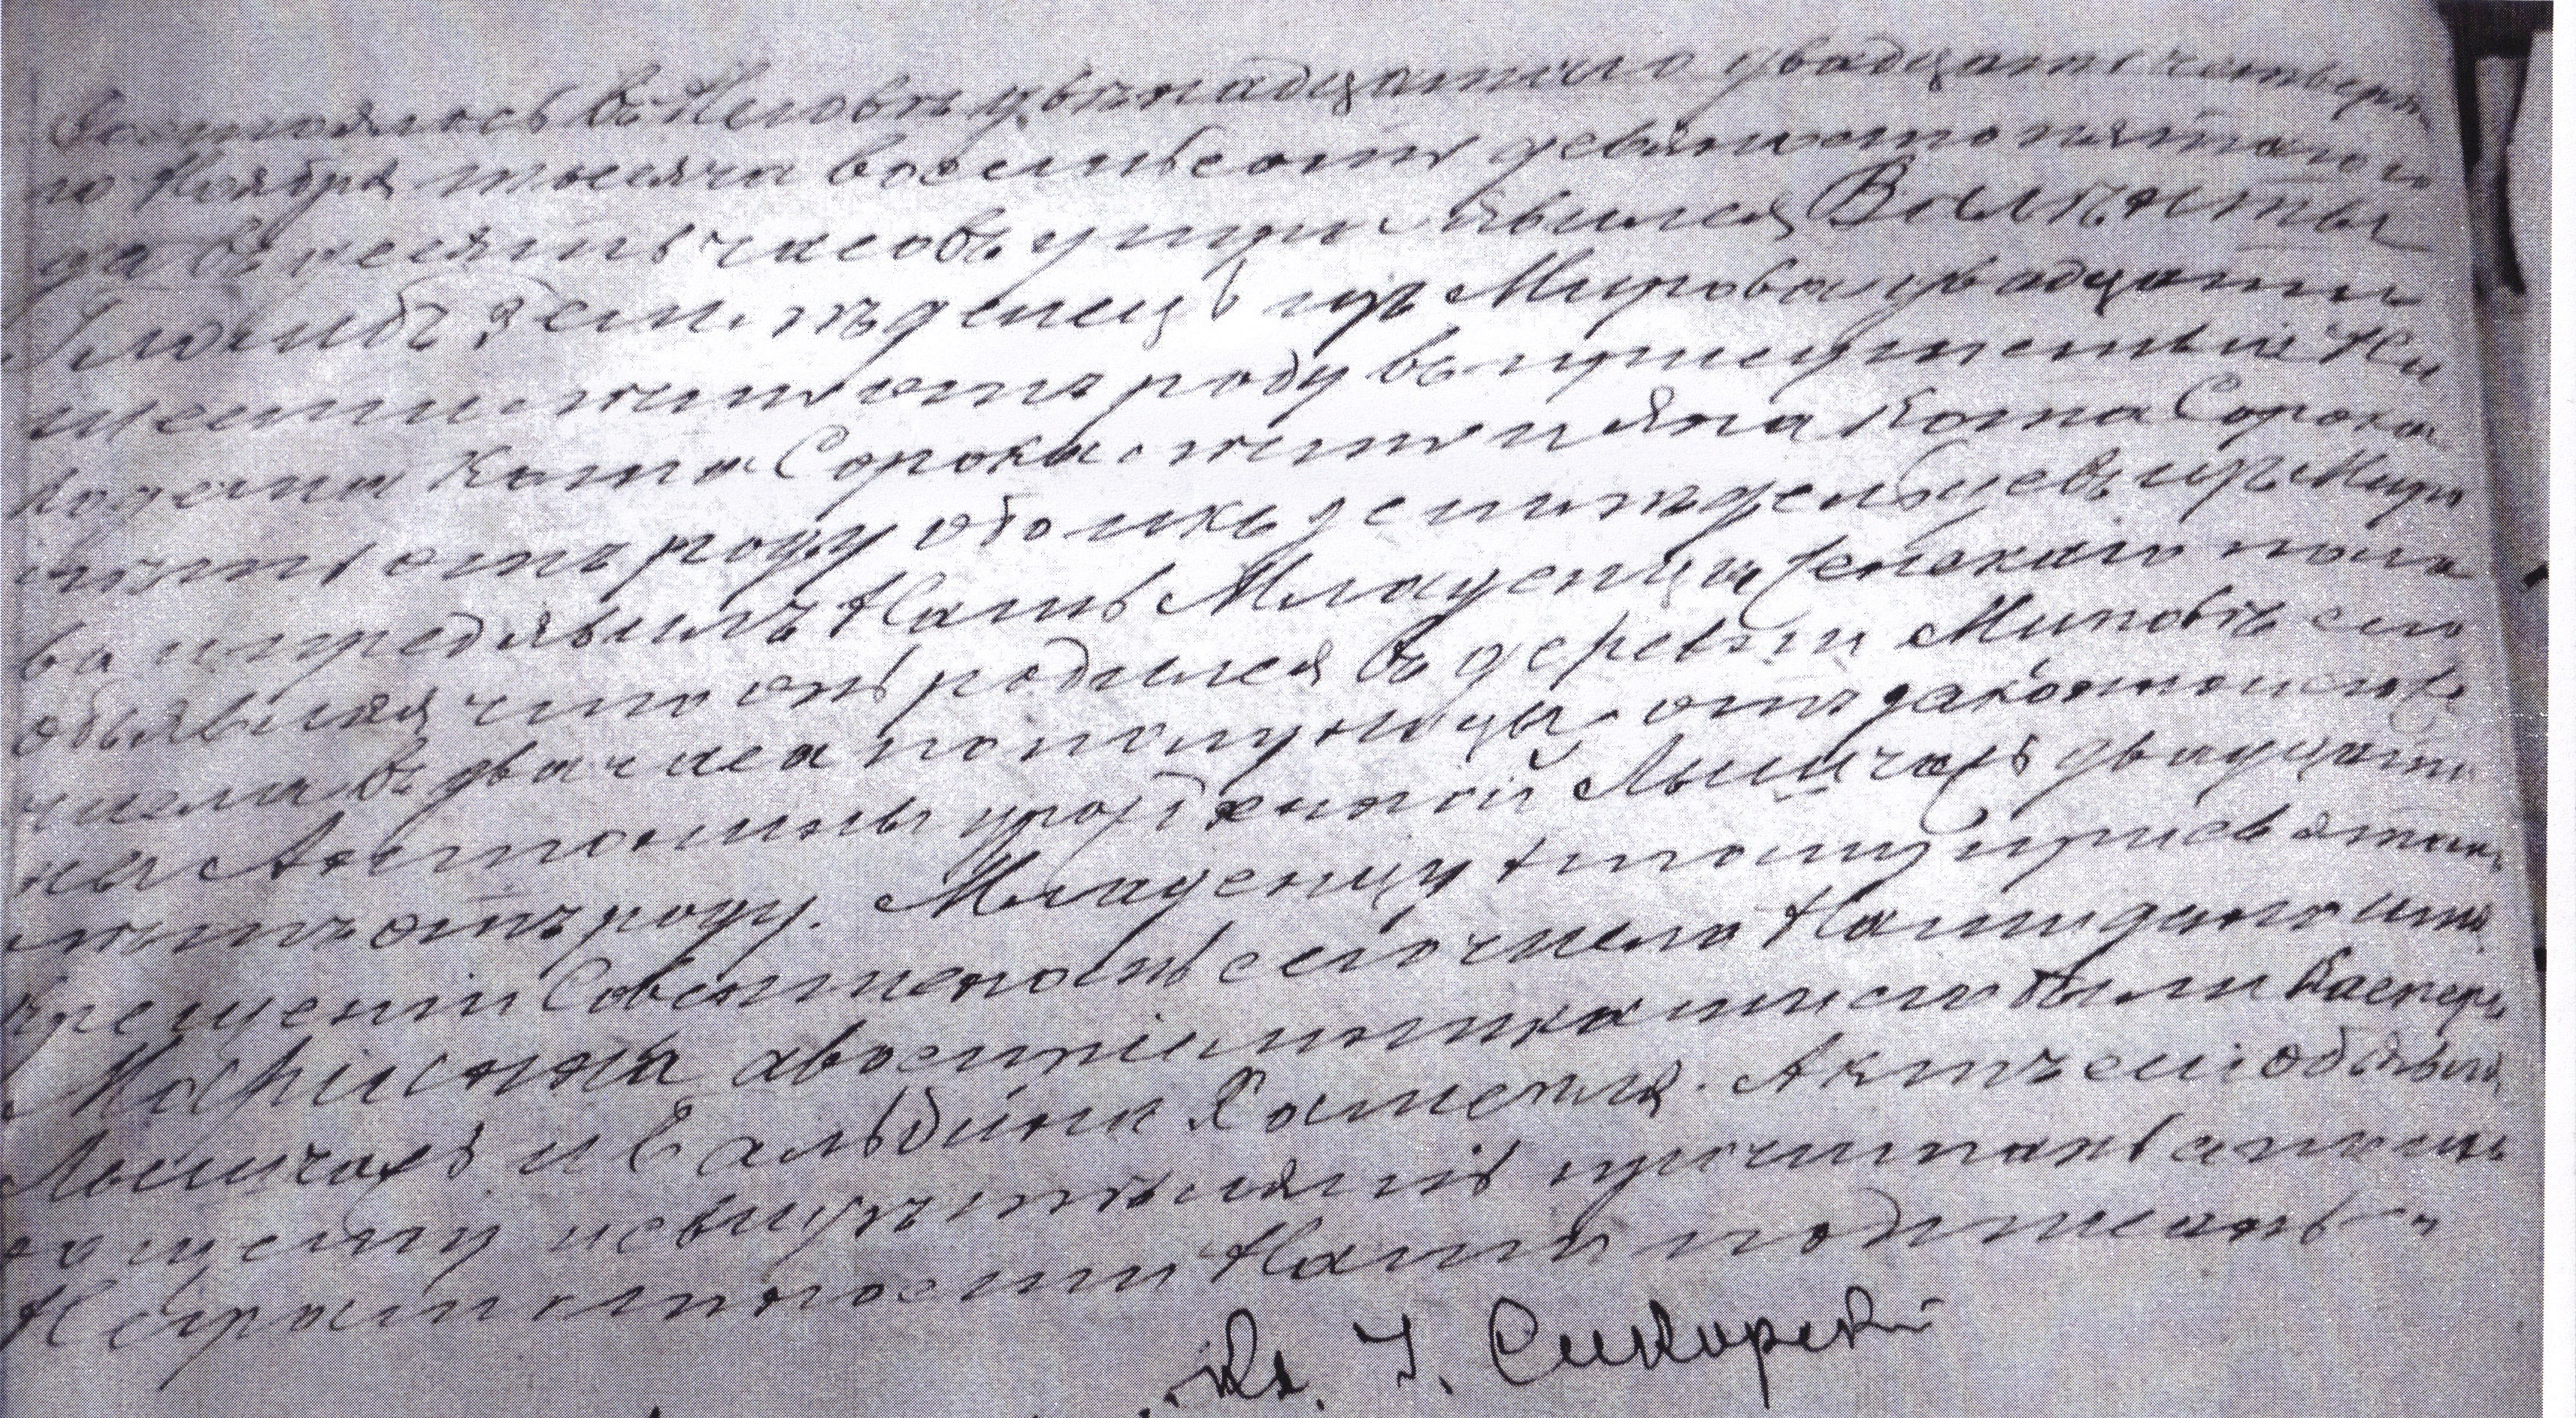
\includegraphics[width=0.8\textwidth]{zdjecia/akt_urodzenia_marianny_glab.jpg}
\caption{Akt urodzenia Marianny Głąbówny.}
\label{rys:akt_urodzenia_marianny_glab}
\end{center}
\end{figure}

\begin{figure}[!ht]
\begin{center}
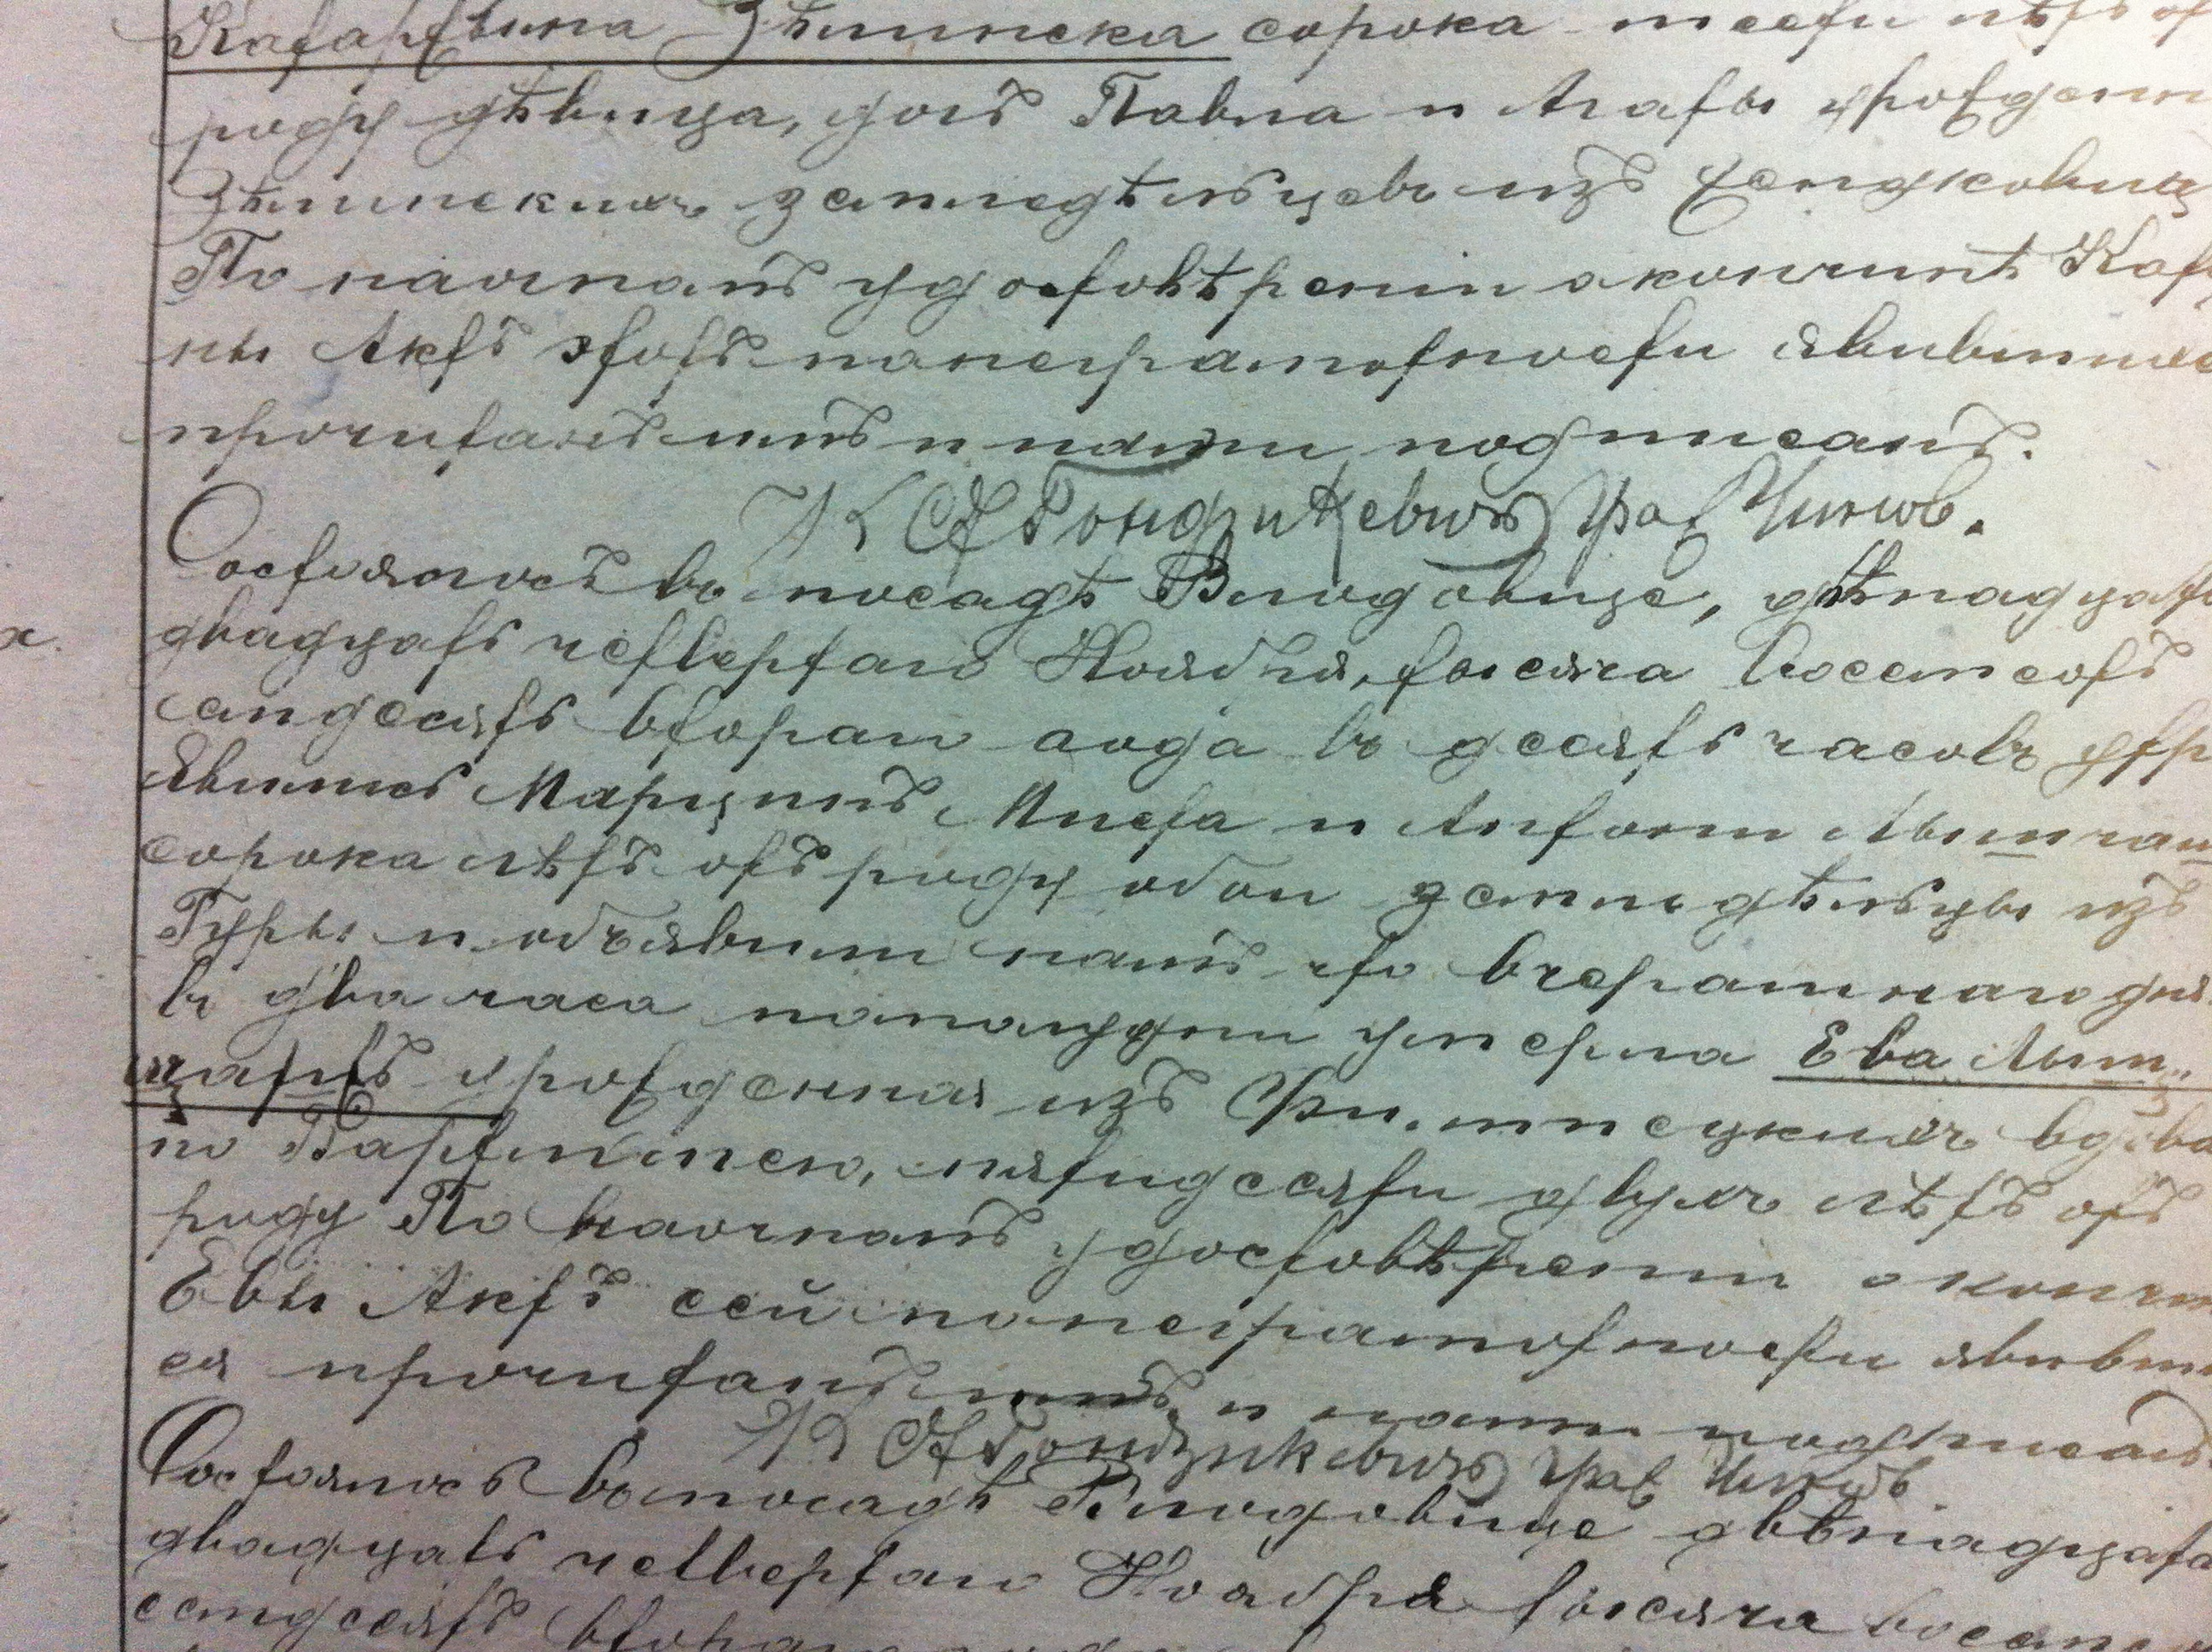
\includegraphics[width=0.73\textwidth]{zdjecia/akt_slubu_sylwestra_gradzika_i_marianny_glab.jpg}
\caption{Akt ślubu Sylwestra Gradzika i Marianny Głąb.}
\label{rys:akt_slubu_sylwestra_gradzika_i_marianny_glab}
\end{center}
\end{figure}

\begin{figure}[!hb]
\begin{center}
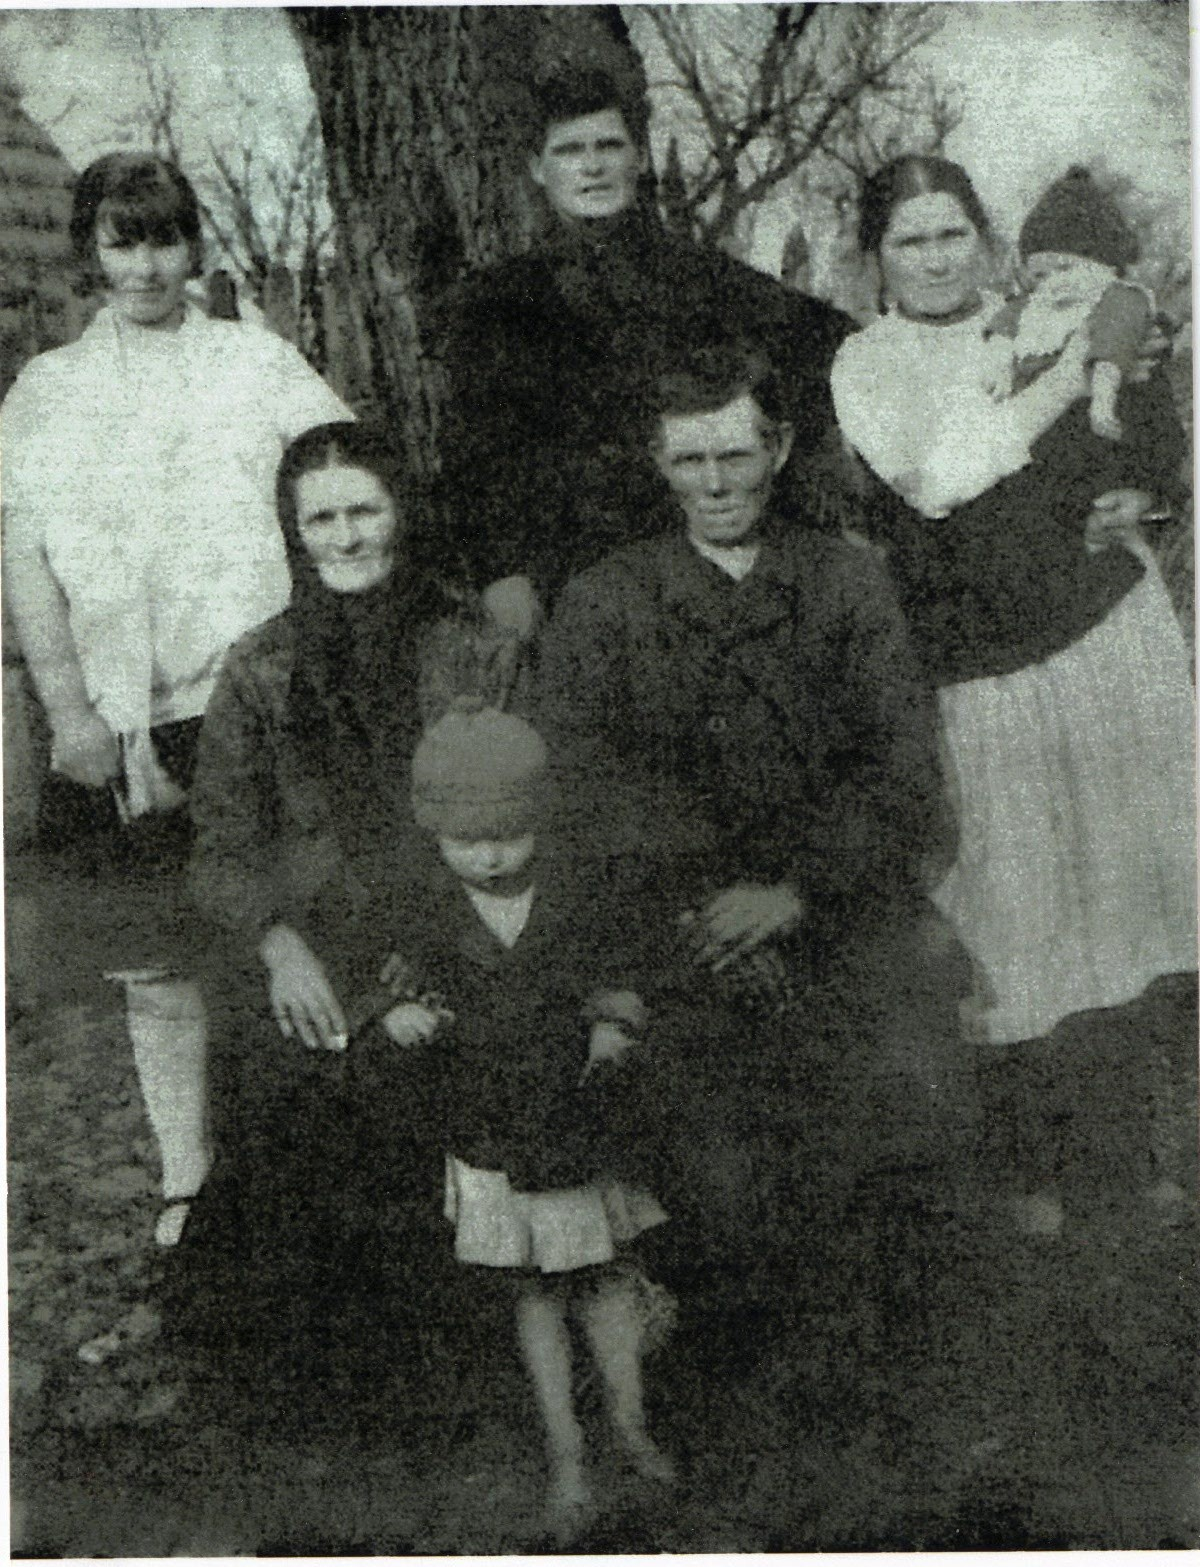
\includegraphics[width=0.47\textwidth]{zdjecia/walenty_antonina_marianna_olimpia.jpg}
\caption[Walenty i Antonina Głąbowie z dziećmi: Bolesławą, Franciszkiem i Marianną Gradzik z jej córkami: Olimpią i Genowefą]{Walenty i Antonina Głąbowie (siedzący) ze swoimi dziećmi: Bolesławą (z lewej), Franciszkiem (obok) i Marianną Gradzik z wnuczkami: Olimpią (na pierwszym planie) i Genowefą (na rękach)}
\label{rys:walenty_antonina_marianna_olimpia}
\end{center}
\end{figure}

O jej rękę ubiegał się Sylwester Gradzik (ur. w~Mirowie 30 XII 1889~r., syn Kazimierza i~Salomei z~Bialików), za którego wyszła dnia 1 X 1917~r. w Niegowie (rys.~\ref{rys:akt_slubu_sylwestra_gradzika_i_marianny_glab}).

Miała z nim córkę Olimpię Gradzik (ur. 13 XI 1919 r. w Mirowie), córkę Genowefę Gradzik (ur.~31~I~1924~r. w~Mirowie) oraz syna Bronisława Gradzika (ur. 20 VII 1928~r. w~Mirowie).

\section{Olimpia Gradzik-Lenartowicz}
Olimpia Gradzik wyszła dnia 8 III 1943 r. w Niegowie za Edwarda Lenartowicza (ur. 17 VII 1909~r. w~Hucisku, syna Antoniego i Antoniny z Głąbów) i miała z nim troje dzieci: Mieczysławę Lenartowicz (ur. 6 I 1944 r. w Mirowie), Jana Lenartowicza (ur. 10 IX 1946 r. w Mirowie) oraz Piotra Lenartowicza (ur. 14 VI  1955 r. w Mirowie) (rys.~\ref{rys:olimpia_edward_lenartowicz_z_dziecmi.jpg}). Owa Antonina z Głąbów, matka Edwarda Lenartowicza była córką Sebastiana Głąba (wówczas pisanego jako Sobestian, stąd zdrobnienie ,,Sobek''), brata Walentego Głąba, więc Olimpia Gradzik wyszła za swego kuzyna, wnuka brata swego dziadka!

\begin{figure}[!h]
\begin{center}
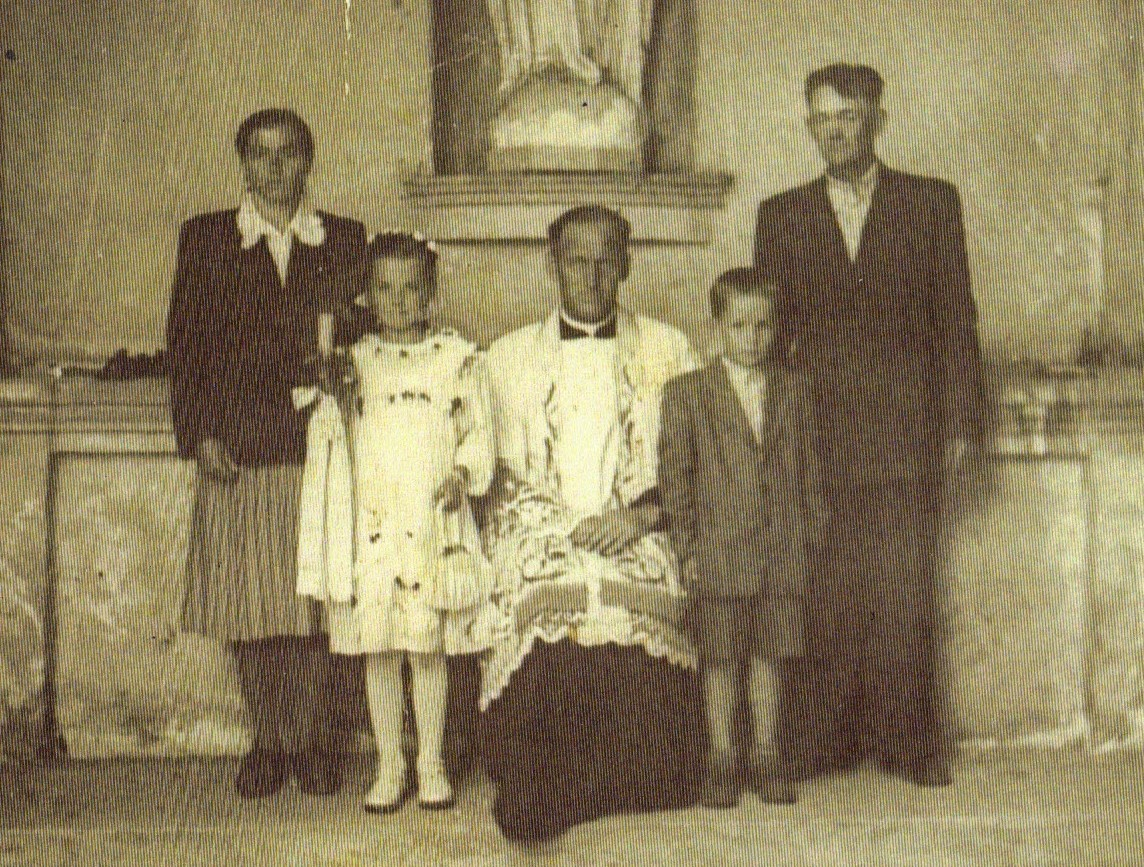
\includegraphics[width=0.6\textwidth]{zdjecia/olimpia_edward_lenartowicz_z_dziecmi.jpg}
\caption[Pierwsza Komunia św. Mieczysławy Lenartowicz, zdjęcie z bratem Janem i rodzicami: Olimpią i Edwardem.]{Pierwsza Komunia Św. Mieczysławy Lenartowicz. Obok księdza stoi młodszy brat Jan, a z tyłu rodzice: Olimpia i Edward Lenartowiczowie}
\label{rys:olimpia_edward_lenartowicz_z_dziecmi.jpg}
\end{center}
\end{figure}

\begin{figure}[!b]
\begin{center}
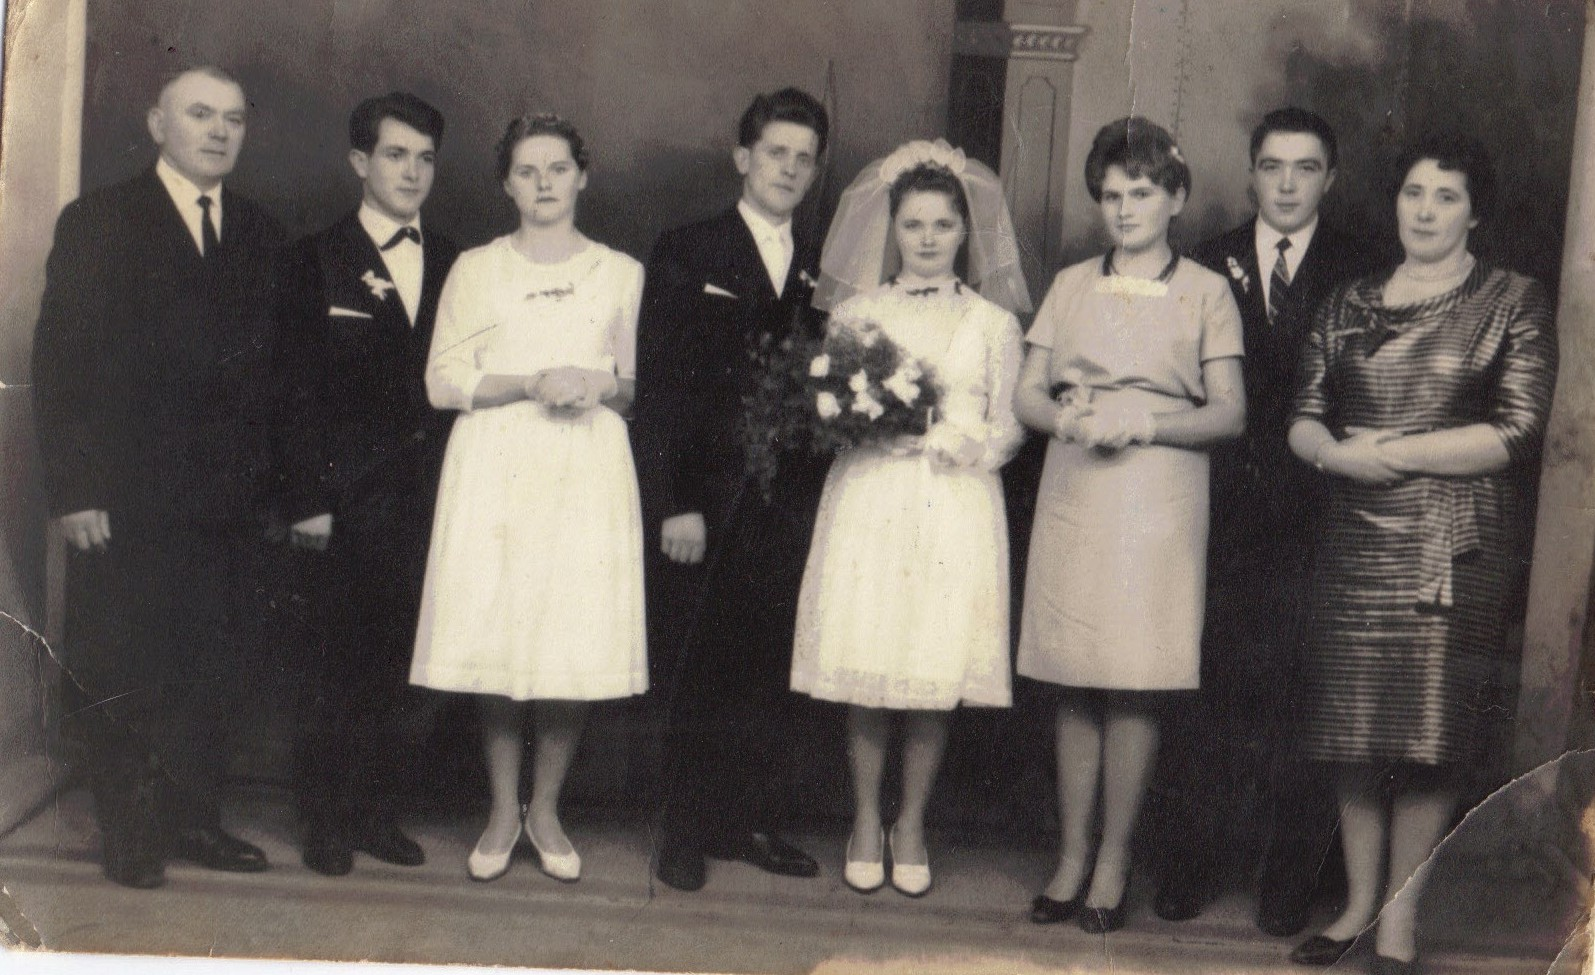
\includegraphics[width=0.7\textwidth]{zdjecia/slub_mieczyslawy_i_mariana_szczepanczykow.jpg}
\caption[Ślub Mieczysławy i Mariana Szczepańczyków]{Ślub Mieczysławy i Mariana Szczepańczyków. Od lewej: Wacław Bubel, starszy drużba ze strony Mariana, starsza druhna -- siostra Mariana (obecnie siostra zakonna), Młoda Para, Anna Kurek, Longin Bubel i jego matka Eleonora Bubel z domu Karoń}
\label{rys:slub_mieczyslawy_i_mariana_szczepanczykow}
\end{center}
\end{figure}

Mieczysława Lenartowicz wyszła dnia 5 V 1963~r. za Mariana Szczepańczyka (ur. 30 I 1933~r. w~Jaworzniku) (rys.~\ref{rys:slub_mieczyslawy_i_mariana_szczepanczykow}), z którym ma troje dzieci: Roberta Szczepańczyka (ur. 10 VIII 1964~r. w Myszkowie), Mariolę Szczepańczyk (ur. 6 I 1966~r. w Myszkowie) oraz Edytę Szczepańczyk (ur. 22 XI 1977 r. w~Myszkowie). Edyta wyszła za Mariusza Pisarskiego (ur.4 II 1973 r. w Zawierciu), z którym ma dwie córki: Wiktorię ur. dnia 27 IX 2006 r. w Myszkowie oraz Olgę ur. dnia 17 VII 2012 r. w Myszkowie. Marian Szczepańczyk zmarł 26 II 2012 r. w Myszkowie.

Jan Lenartowicz ożenił się dnia 5 II 1983 r. w Zawierciu z Czesławą Pańczyk ur. dnia 7 IX 1952~r. w~Zawierciu i ma z nią dwoje dzieci: syna Rafała Lenartowicza ur. dnia 30 IV 1983 r. w Zawierciu i córkę Dorotę Lenartowicz ur. dnia 15 VII 1984~r. w Zawierciu (rys.~\ref{rys:dorota_lenartowicz_z_synem_frankiem}). Dorota Lenartowicz wyszła 28 XI  2009 r. za Mariusza Sołtysika, z którym ma syna Franciszka urodzonego 4 V 2009 r. w Zawierciu.

\begin{figure}[!ht]
\begin{center}
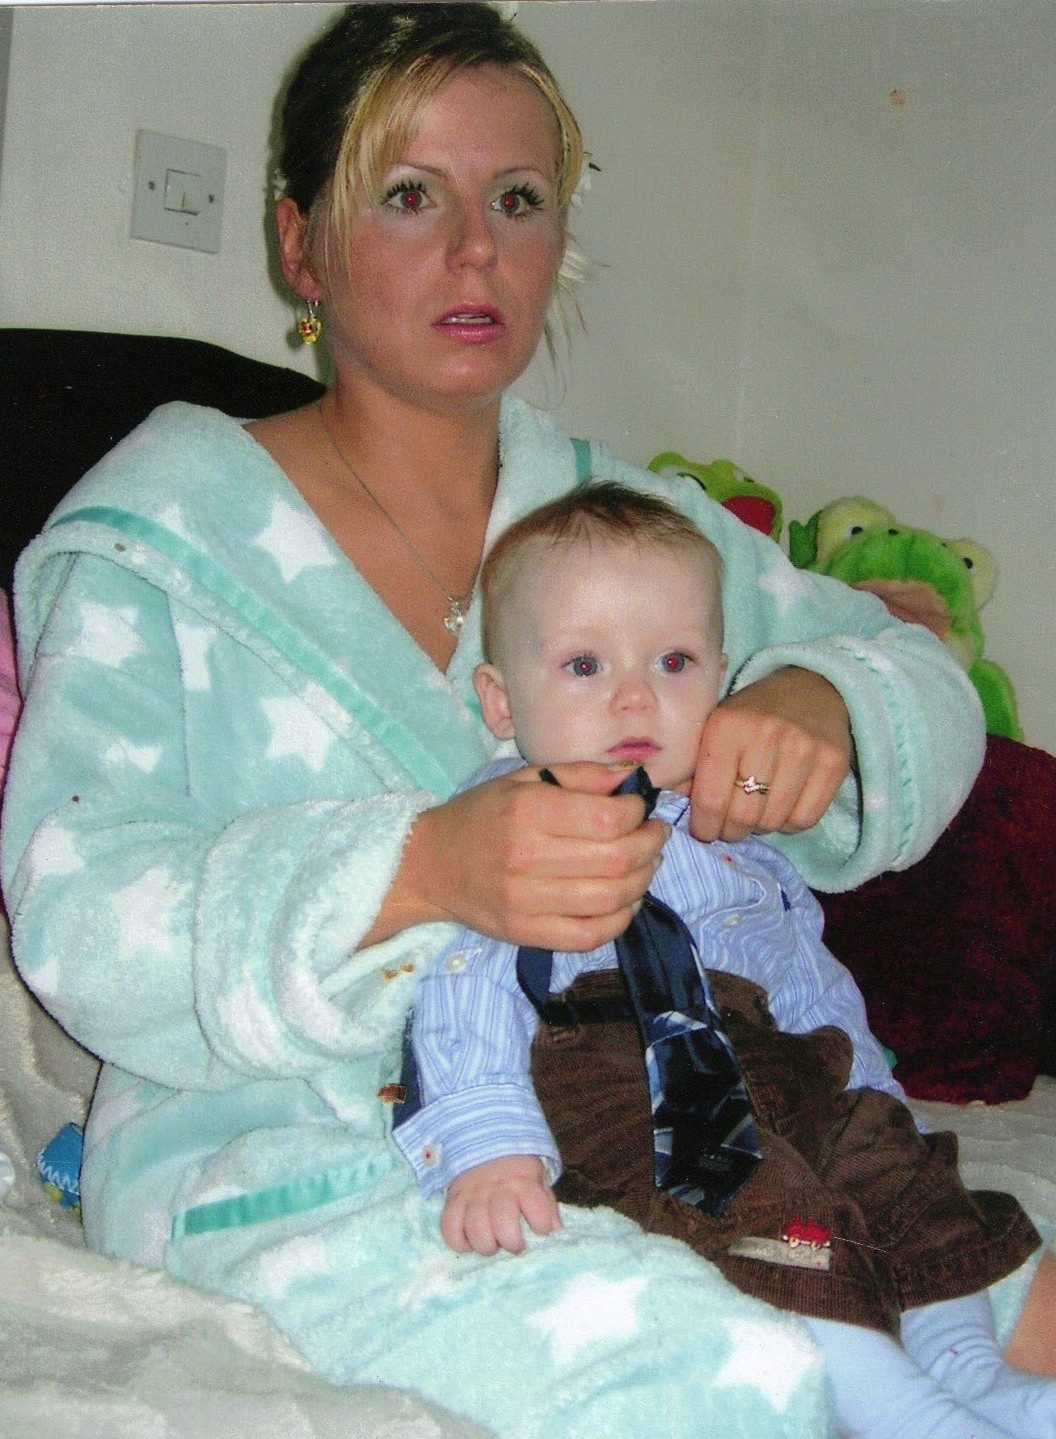
\includegraphics[width=0.3\textwidth]{zdjecia/dorota_lenartowicz_z_synem_frankiem.jpg}
\caption{Dorota Lenartowicz-Sołtysik z synem Frankiem}
\label{rys:dorota_lenartowicz_z_synem_frankiem}
\end{center}
\end{figure}

\begin{figure}[!h]
\begin{center}
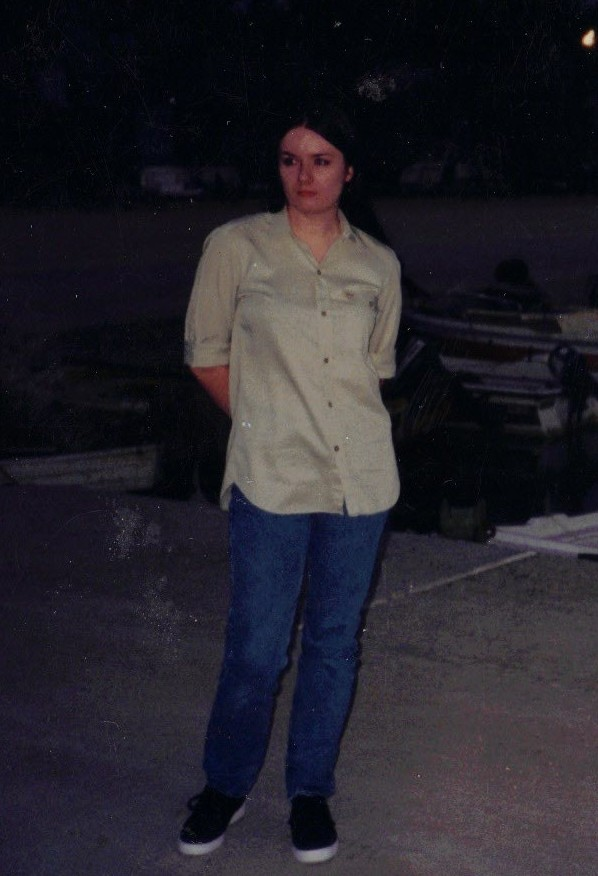
\includegraphics[width=0.3\textwidth]{zdjecia/dagmara_lenartowicz_podaras.jpg}
\caption{Dagmara Podaras (z domu Lenartowicz)}
\label{rys:dagmara_lenartowicz_podaras}
\end{center}
\end{figure}

Piotr Lenartowicz ożenił się w lipcu 1978 r. we Wrzosowej z Jagodą Nagodą ur. dnia 4~XII~1955~r. w Częstochowie i ma z nią dwoje dzieci: córkę Dagmarę Lenartowicz ur. dnia 11~V~1979~r. w Częstochowie (rys.~\ref{rys:dagmara_lenartowicz_podaras}) i syna Łukasza Lenartowicza ur. 28~V~1980~r. w~Częstochowie. Dagmara wyszła w Patras dnia 23 X 2004~r. za rodowitego Greka Afanasija Podarasa i ma z~nim córkę Stellę Podaras ur. 14 VIII 2005~r. w Atenach.



\section{Genowefa Gradzik-Surowiec}
Genowefa Gradzik wyszła dnia 15 IX 1946 r. za Władysława Surowca (ur. 5 VI 1921 r. w Mirowie z ojca Wojciecha i matki Anieli z domu Kurek). Z tego małżeństwa zrodziło się sześcioro dzieci, pięcioro z nich zmarło we wczesnym okresie niemowlęctwa, żyje tylko najmłodsza córka Ewa Zofia Surowiec (ur. 5 IV 1954~r. w~Mirowie) (rys.~\ref{rys:ewa_skowronek_genowefa_i_wladyslaw_surowiec}).


\begin{figure}[!h]
\begin{center}
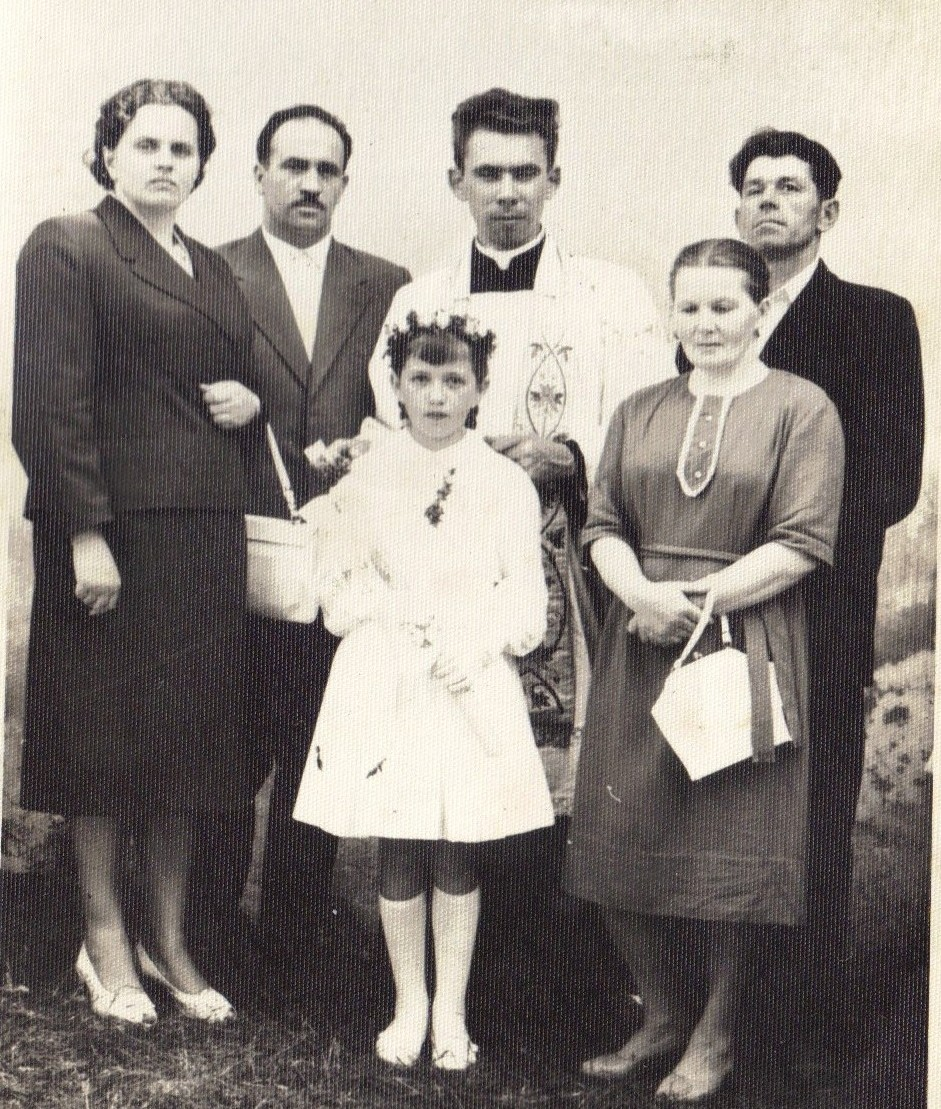
\includegraphics[width=0.47\textwidth]{zdjecia/ewa_skowronek_genowefa_i_wladyslaw_surowiec.jpg}
\caption[Pierwsza Komunia św. Ewy Surowiec]{Pierwsza Komunia św. Ewy Surowiec, prawnuczki Antoniny i Walentego Głąbów. Z lewej Maria i Władysław Bublowie jako chrzestni. Z prawej Genowefa Surowiec, z domu Gradzik (wnuczka Antoniny i Walentego Głąbów, córka Marianny Głąb-Gradzik) z Władysławem Surowcem}
\label{rys:ewa_skowronek_genowefa_i_wladyslaw_surowiec}
\end{center}
\end{figure}

\begin{figure}[!ht]
\begin{center}
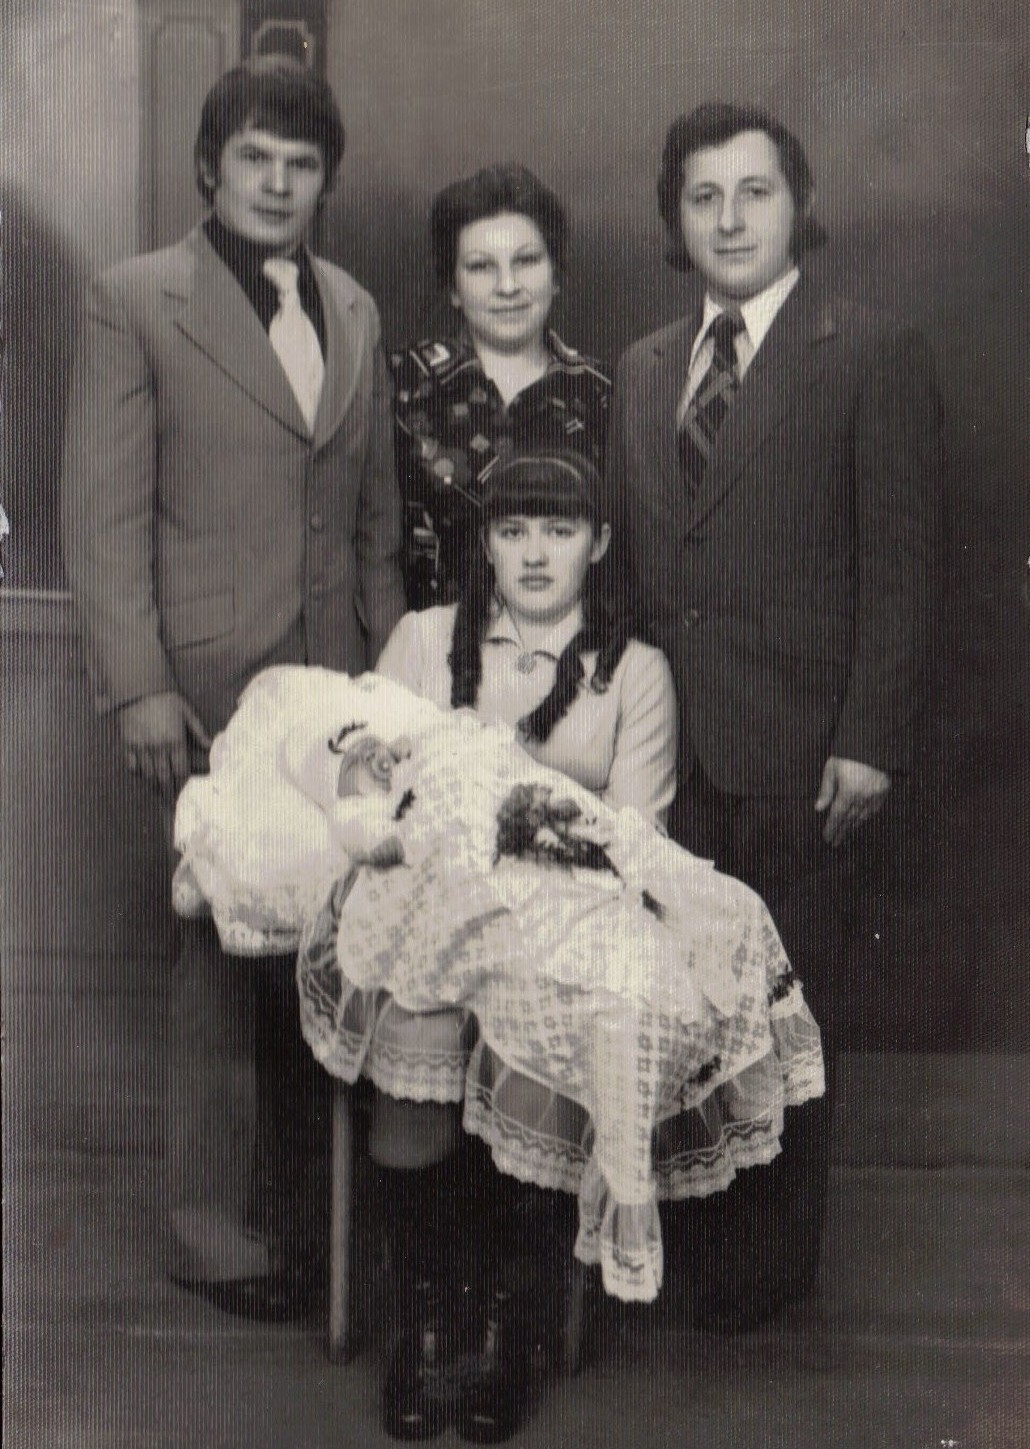
\includegraphics[width=0.4\textwidth]{zdjecia/marcin_skowronek_chrzest.jpg}
\caption[Chrzest św. Marcina Skowronka]{Chrzest św. Marcina Skowronka - prawnuczka Marianny Gradzik z domu Głąb. Z lewej stoją chrzestni: Sylwester Gradzik i Aleksandra Niemczyk, z prawej ojciec Stefan Skowronek. Marcin trzymany na rękach przez mamę Ewę Skowronek.}
\label{rys:marcin_skowronek_chrzest}
\end{center}
\end{figure}

\begin{figure}[!hb]
\begin{center}
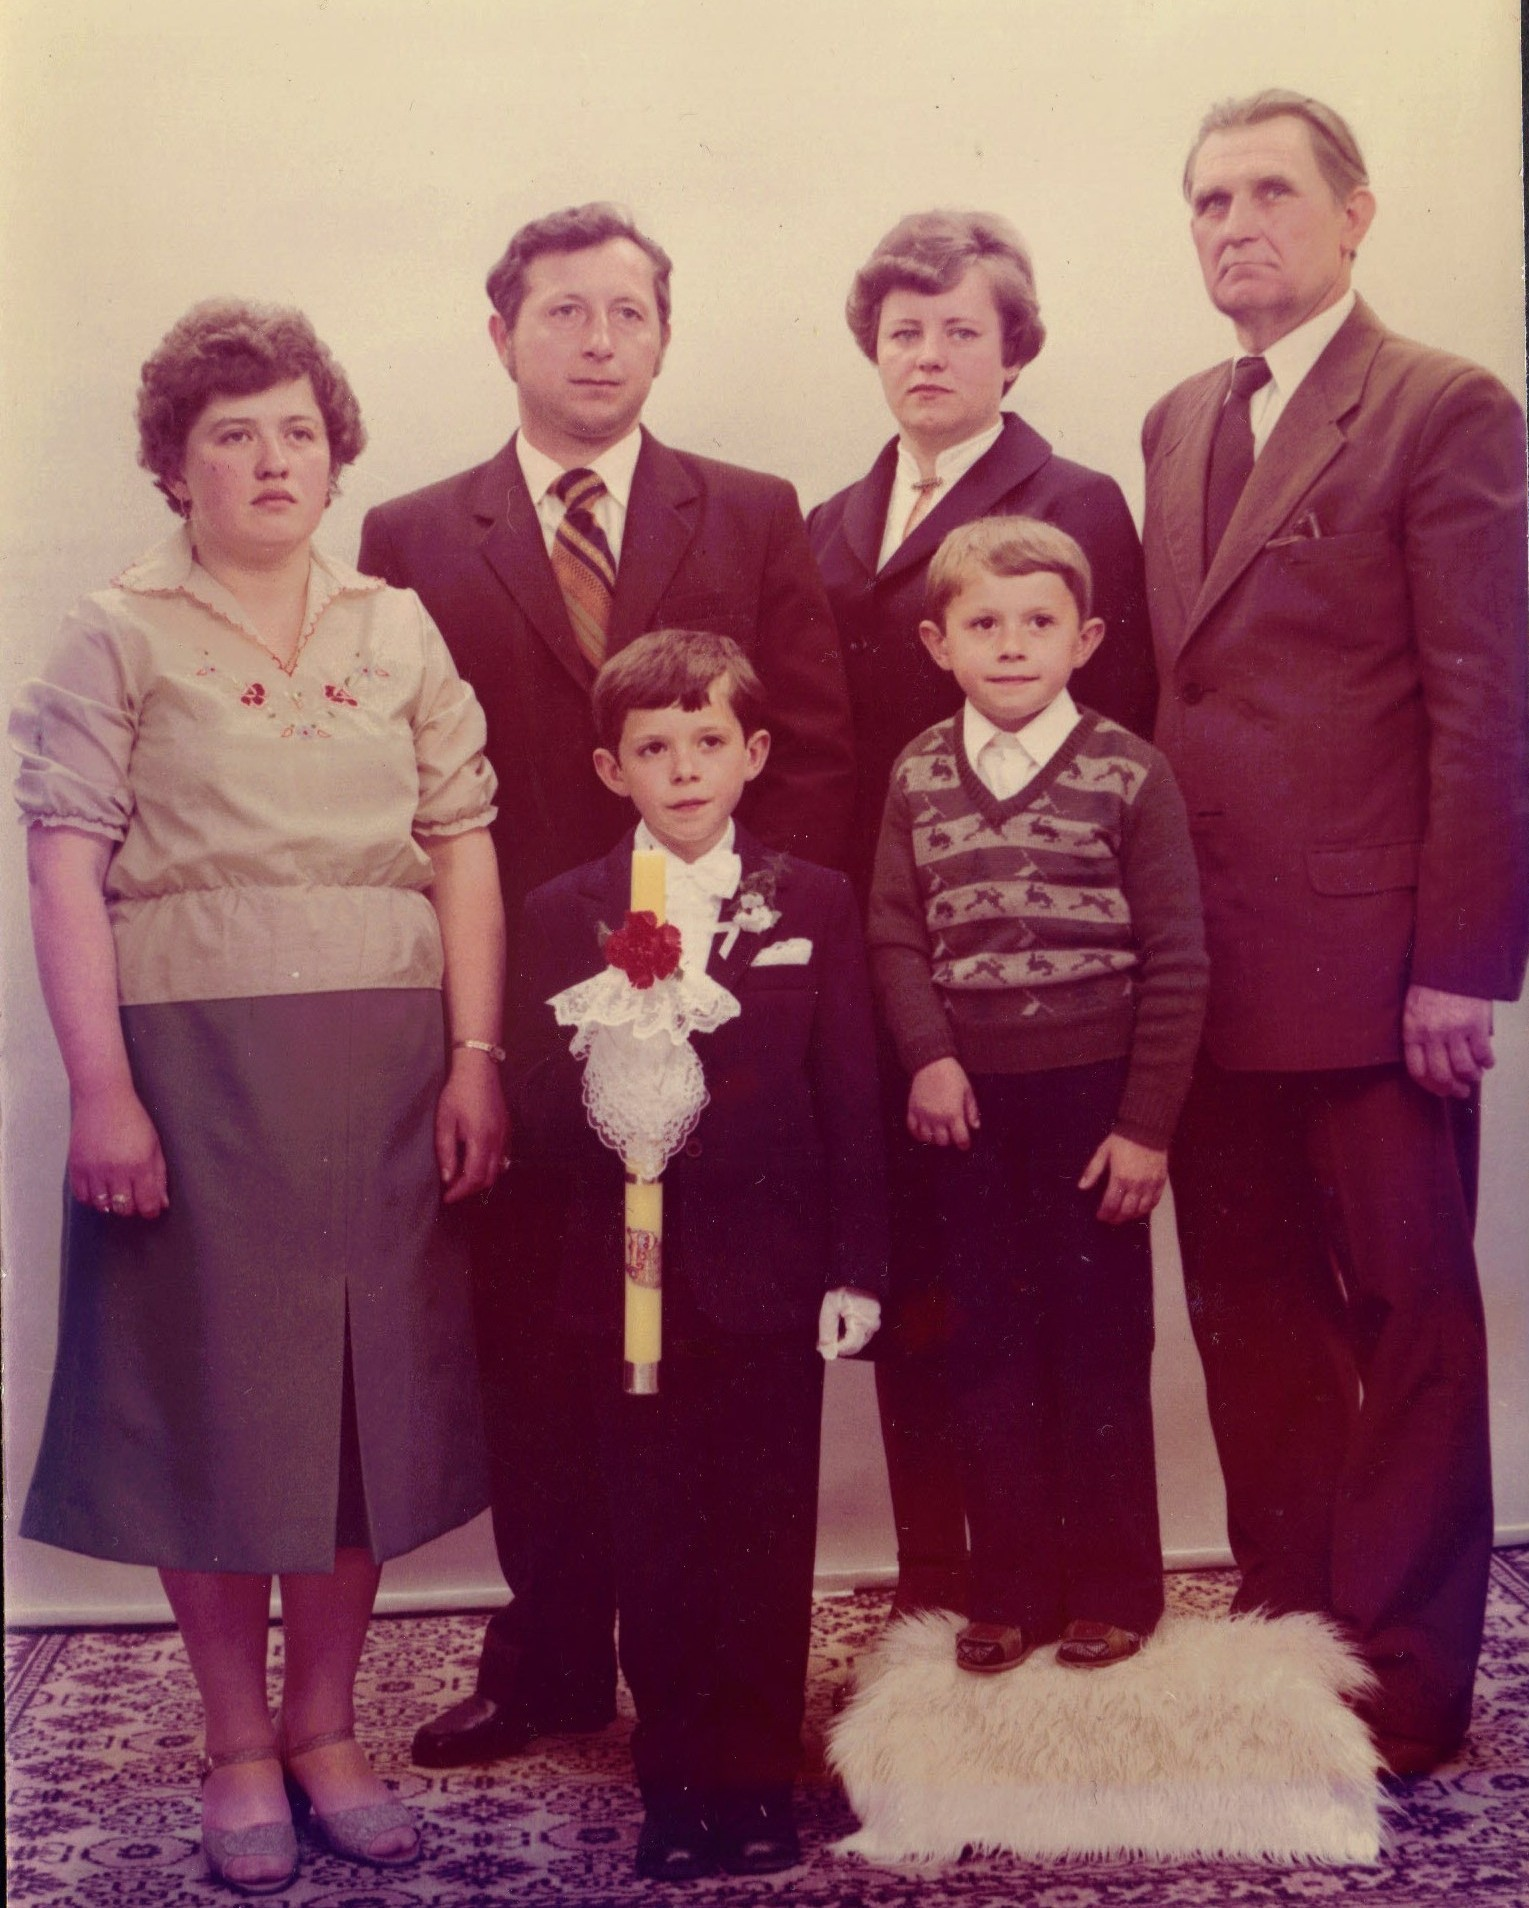
\includegraphics[width=0.43\textwidth]{zdjecia/pawel_skowronek_1_komunia.jpg}
\caption[I Komunia św. Pawła Skowronka]{I Komunia św. Pawła Skowronka - prawnuczka Marianny Gradzik z domu Głąb. Z lewej rodzice (Ewa i Stefan Skowronkowie), z prawej rodzice chrzestni (Anna Skowronek i Zygmunt Maciąg) obok stoi brat Marcin}
\label{rys:pawel_skowronek_1_komunia}
\end{center}
\end{figure}

Wyszła ona dnia 15 IV 1974~r. w Niegowie (ślub odbył się w Mirowie) za Stefana Skowronka (ur. 4 X 1949~r. w Zawierciu z ojca Konstantego i matki Stefanii z Pasierbów) i ma z nim dwóch synów: Pawła (ur. 25 VIII 1974 r. w Myszkowie) (rys.~\ref{rys:pawel_skowronek_1_komunia}) oraz Marcina (rys.~\ref{rys:marcin_skowronek_chrzest}). Stefan Skowronek zmarł 10~III~2014~r. w szpitalu w Zabrzu. Miał piękny pogrzeb w Mirowie,  miał bowiem wielu przyjaciół i był radnym Rady Gminy Niegowa.

\begin{figure}[!t]
\begin{center}
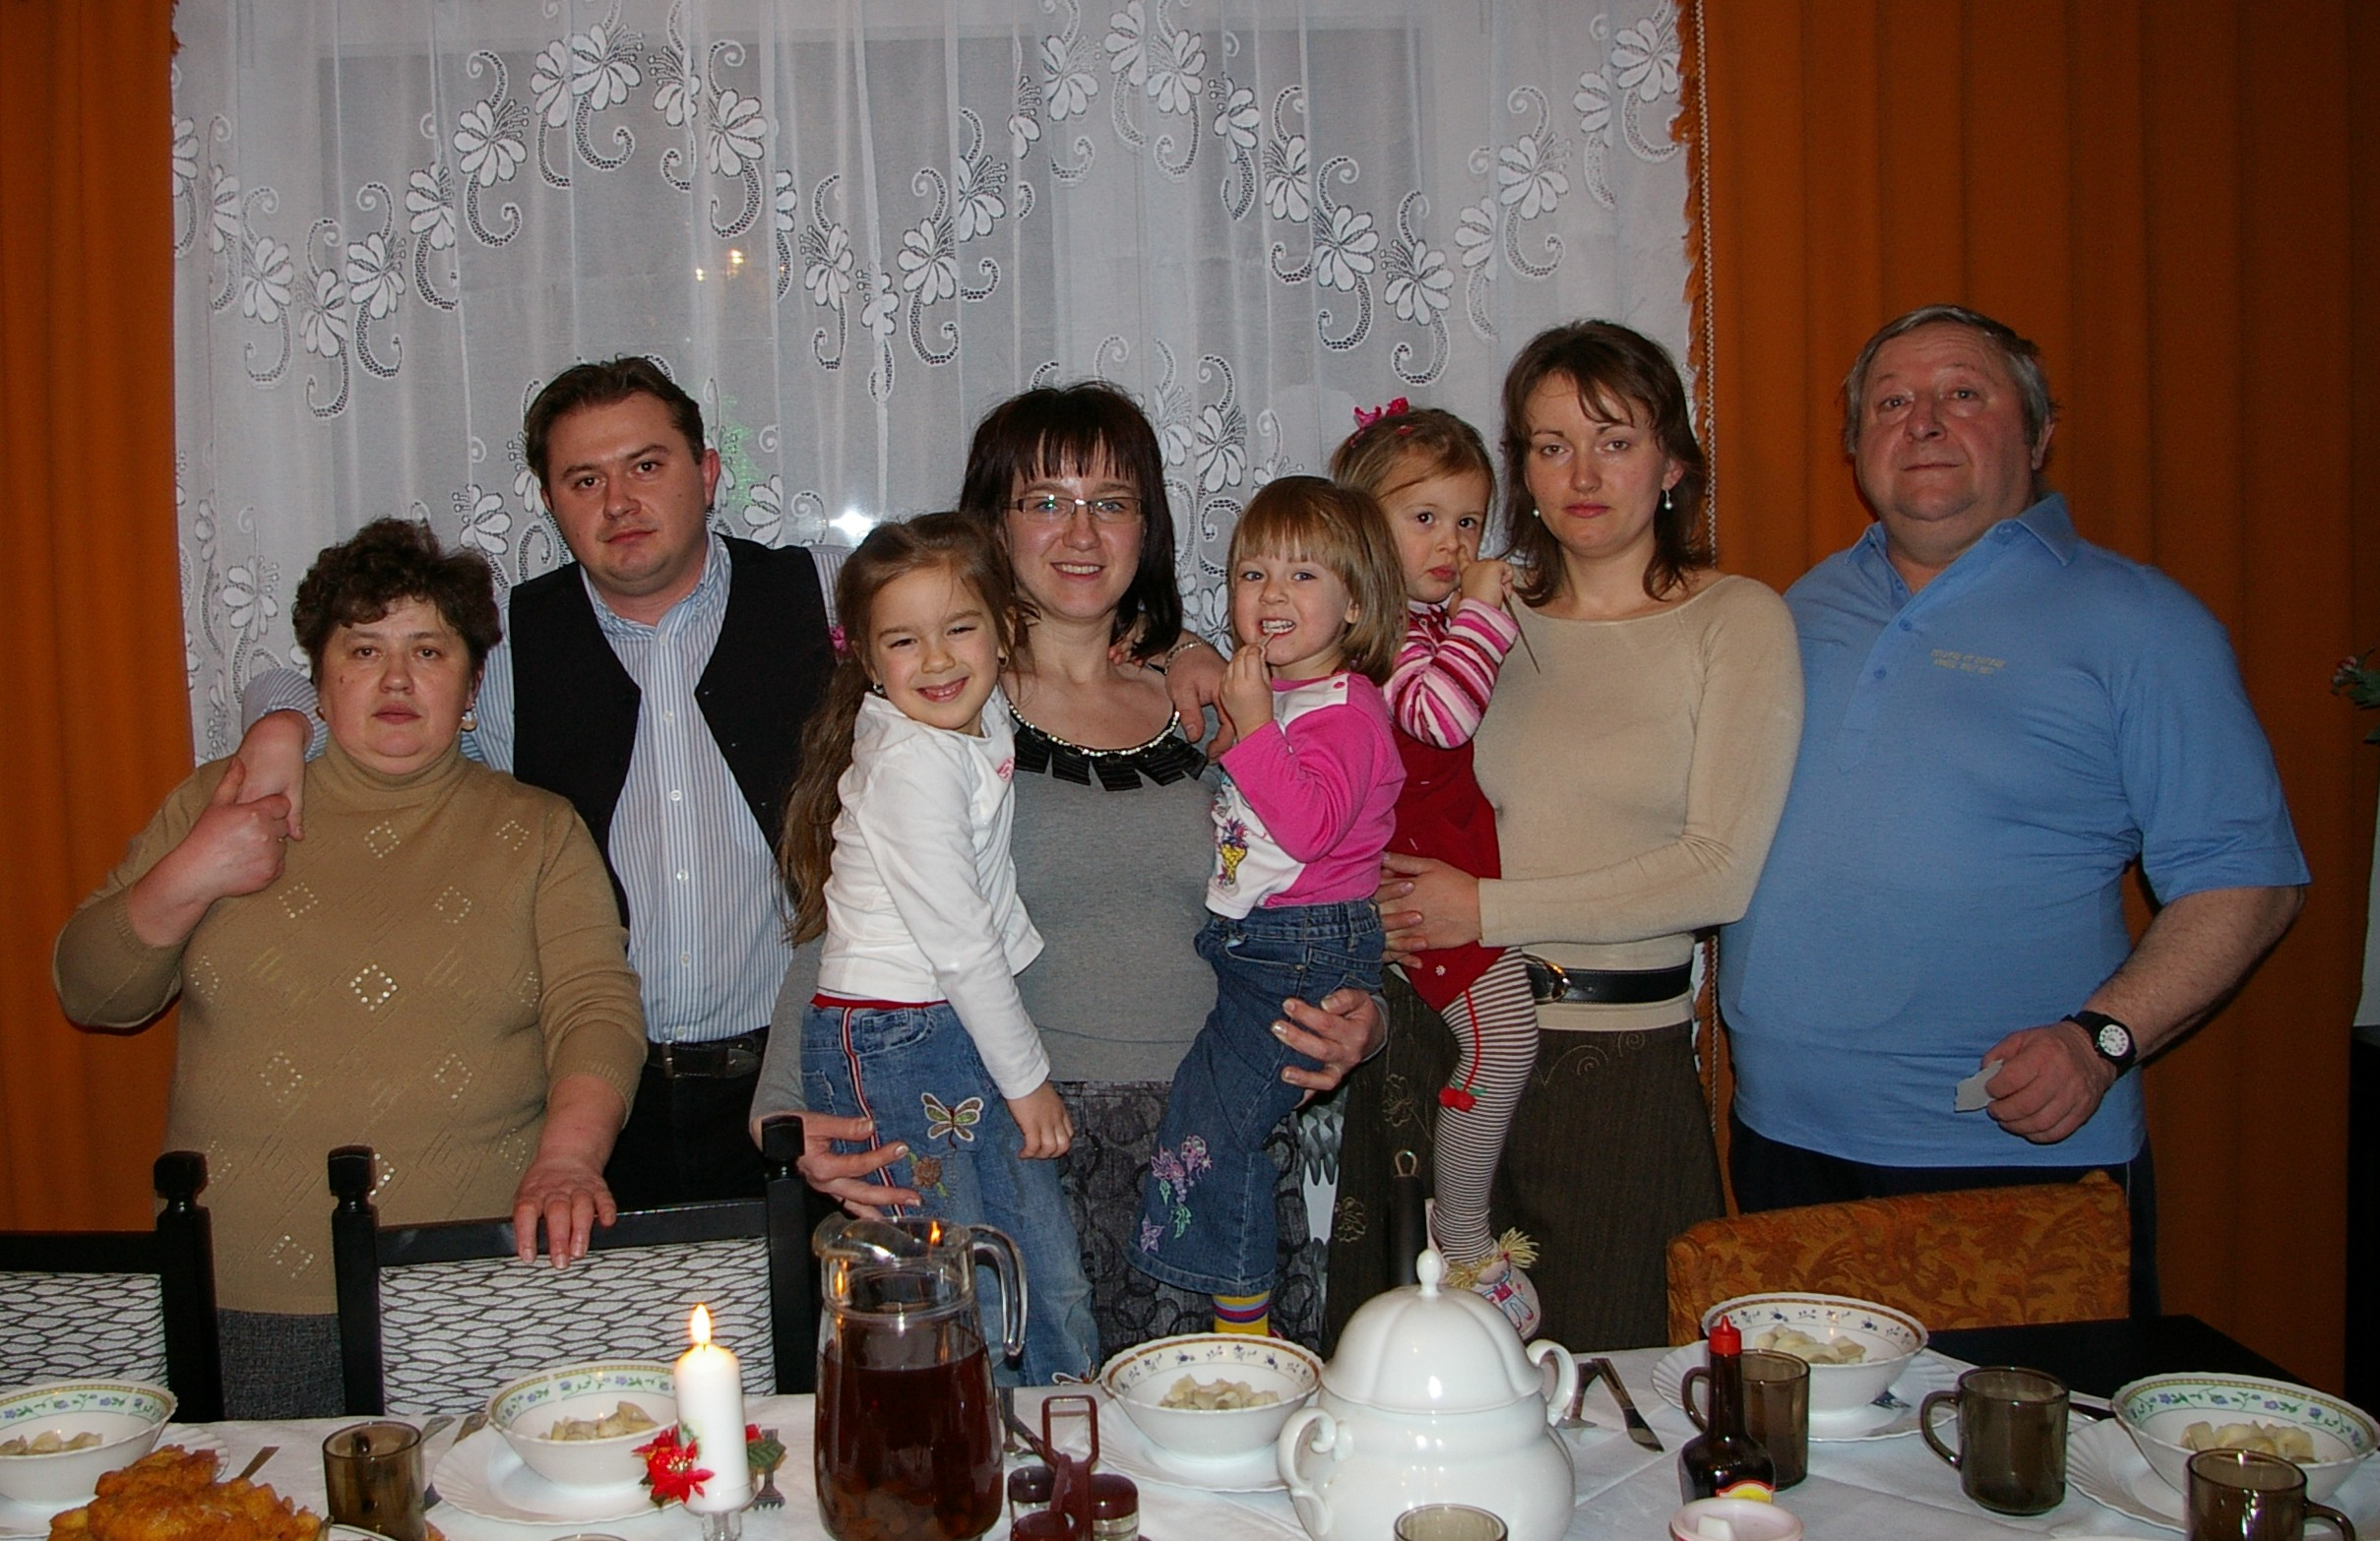
\includegraphics[width=\textwidth]{zdjecia/rodzina_skowronkow_1.jpg}
\caption[Rodzina Skowronków]{Rodzina Skowronków. Od lewej stoją: Ewa Skowronek (wnuczka Marianny Gradzik z domu Głąb), jej syn Marcin, żona Pawła Skowronka -- Aneta trzymająca córki: Paulinę i Patrycję, dalej żona Marcina -- Małgorzata z córką Agatą i po prawej Stefan Skowronek}
\label{rys:rodzina_skowronkow_1}
\end{center}
\end{figure}

\begin{figure}[!b]
\begin{center}
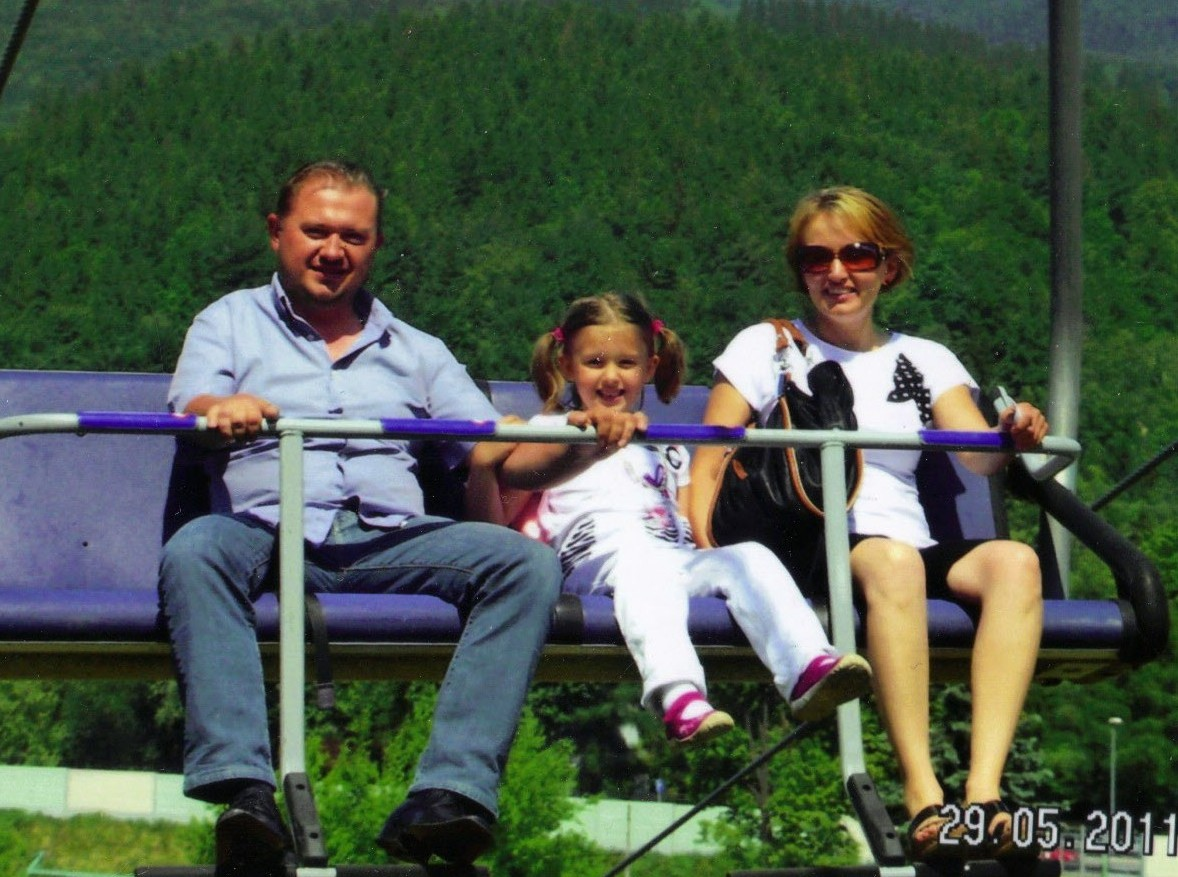
\includegraphics[width=0.65\textwidth]{zdjecia/malgorzata_marcin_agata_skowronek.jpg}
\caption[Rodzina Marcina Skowronka]{Marcin Skowronek (prawnuczek Marianny Gradzik z domu Głąb) z żoną Małgorzatą i córką Agatą}
\label{rys:malgorzata_marcin_agata_skowronek}
\end{center}
\end{figure}

Marcin urodził się 12 XII 1976 r. niestety w Myszkowie, gdyż tamtejszy oddział położniczy miał jak najgorszą sławę i słusznie. Gdy bowiem Ewa rodziła Marcina cała obsługa medyczna imprezowała suto zakrapiając alkoholem, głucha na jej błagalne wezwania pomocy. Dopiero gdy dzieciątko było już zupełnie sine z niedotlenienia pijany personel zajął się Ewą. Podczas porodu nietrzeźwe położne wyrwały Marcinowi rączkę i usiłowały to ukryć! W efekcie nieleczona od razu kontuzja okazała się w tamtych czasach  trwała.

Paweł Skowronek ożenił się 9 sierpnia 1997 r. z Anetą Kwiecień (ur.21 maja 1975 r. w Myszkowie z ojca Władysława i matki Mirosławy Czyż) z którą ma dwie córki: Paulinę (ur. 14 II 2001 r. w Chicago) i~Patrycję  (ur. 18 I 2005 r. w Chicago).

Marcin Skowronek wraz z ojcem Stefanem wybudowali pod zamkiem hotel i karczmę i z tego dostatnio żyją. Marcin ożenił się 8 lipca 2000 r. z Małgorzatą Duś (ur. 25  III 1976 r. w Koziegłowach z ojca Leonarda i matki Anny z domu Ziajska) i ma z nią córkę Agatę (ur. 2 II 2005 r. w Częstochowie) (rys.~\ref{rys:malgorzata_marcin_agata_skowronek}).


\section{Bronisław Gradzik}
Bronisław Gradzik ożenił się z Reginą Rosikoń (ur. 29 I 1925 r. w Mirowie z ojca Jana i matki Marianny z~domu Gurbała, która zmarła ) i ma z nią czworo dzieci: Marię (ur. 29 II 1950 r. w Mirowie), Sylwestra (ur. 3 XI 1952 r. w Mirowie), Leszka (ur. 18 V 1955 r. w Mirowie) i najmłodszego ich syna Krzysztofa (ur. 1 V 1957 r. w Mirowie). 

\begin{figure}[!h]
\begin{center}
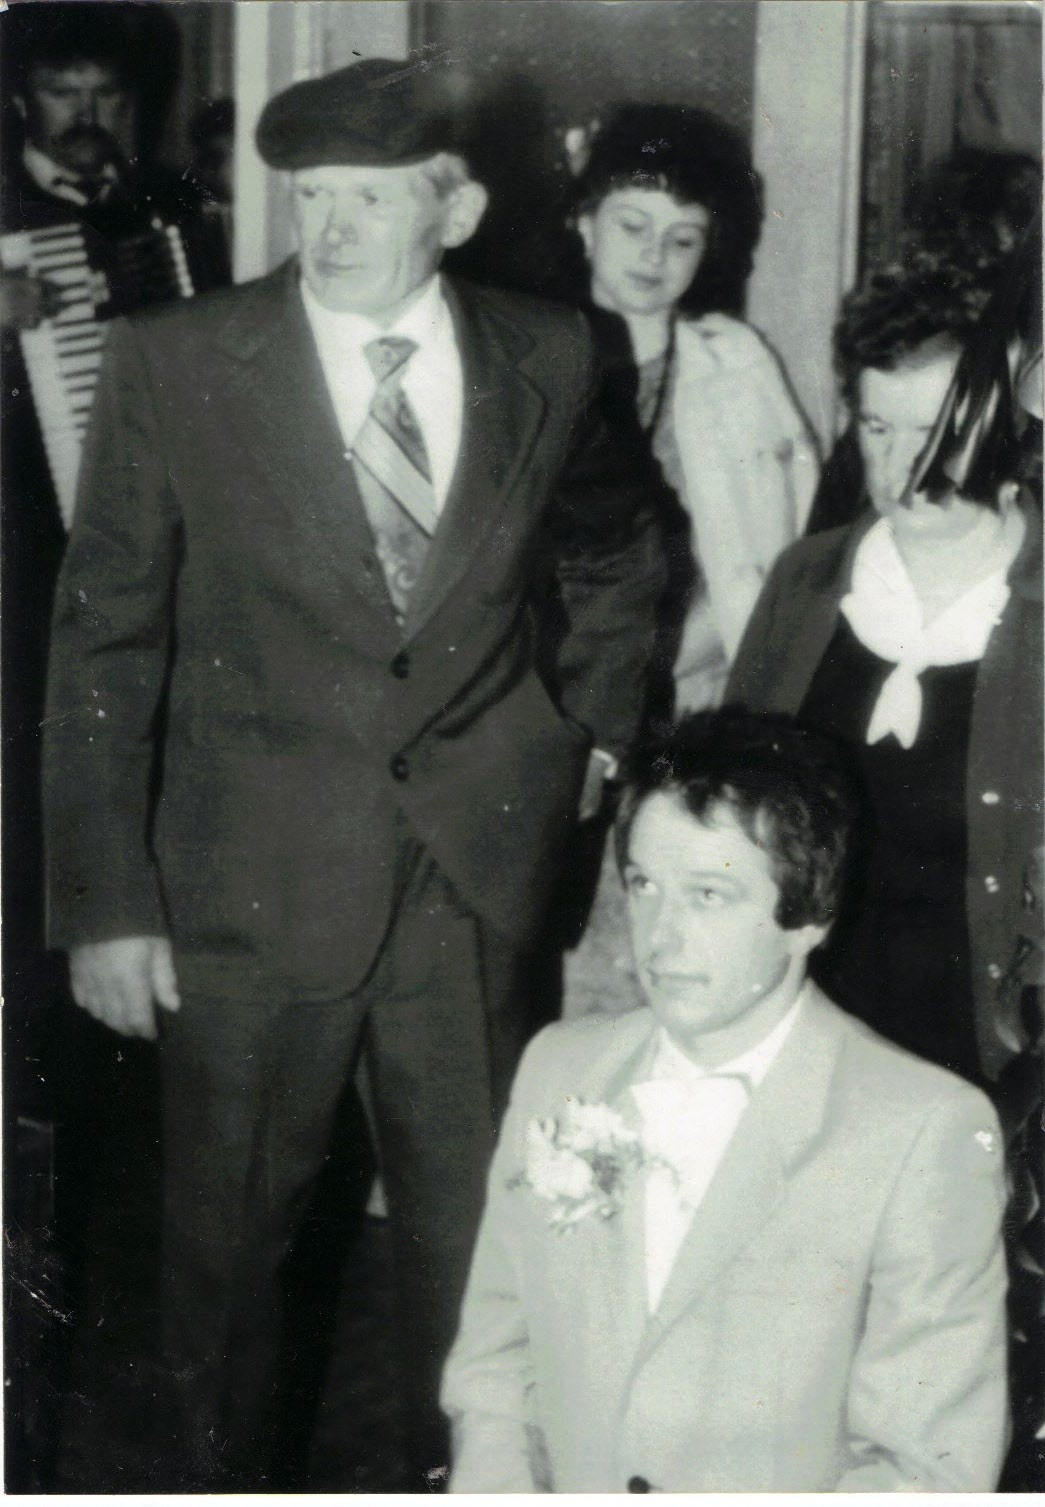
\includegraphics[width=0.5\textwidth]{zdjecia/bronislaw_regina_krzysztof_gradzikowie.jpg}
\caption{Bronisław i Regina Gradzikowie na ślubie ich syna Krzysztofa.}
\label{rys:bronislaw_regina_krzysztof_gradzikowie}
\end{center}
\end{figure}

Najstarsza Maria Gradzikówna wyszła za Zbigniewa Popczyka (ur. 25 IV 1948~r. w Ciągowicach z ojca Stefana i matki Danieli z domu Szewczyk) (rys.~\ref{rys:slub_marii_gradzik_i_marka_popczyka}) i ma z nim córkę Ewelinę oraz syna Damiana (rys.~\ref{rys:damian_maria_ewelina_popczykowie_marcin_gradzik}).

\begin{figure}[!h]
\begin{center}
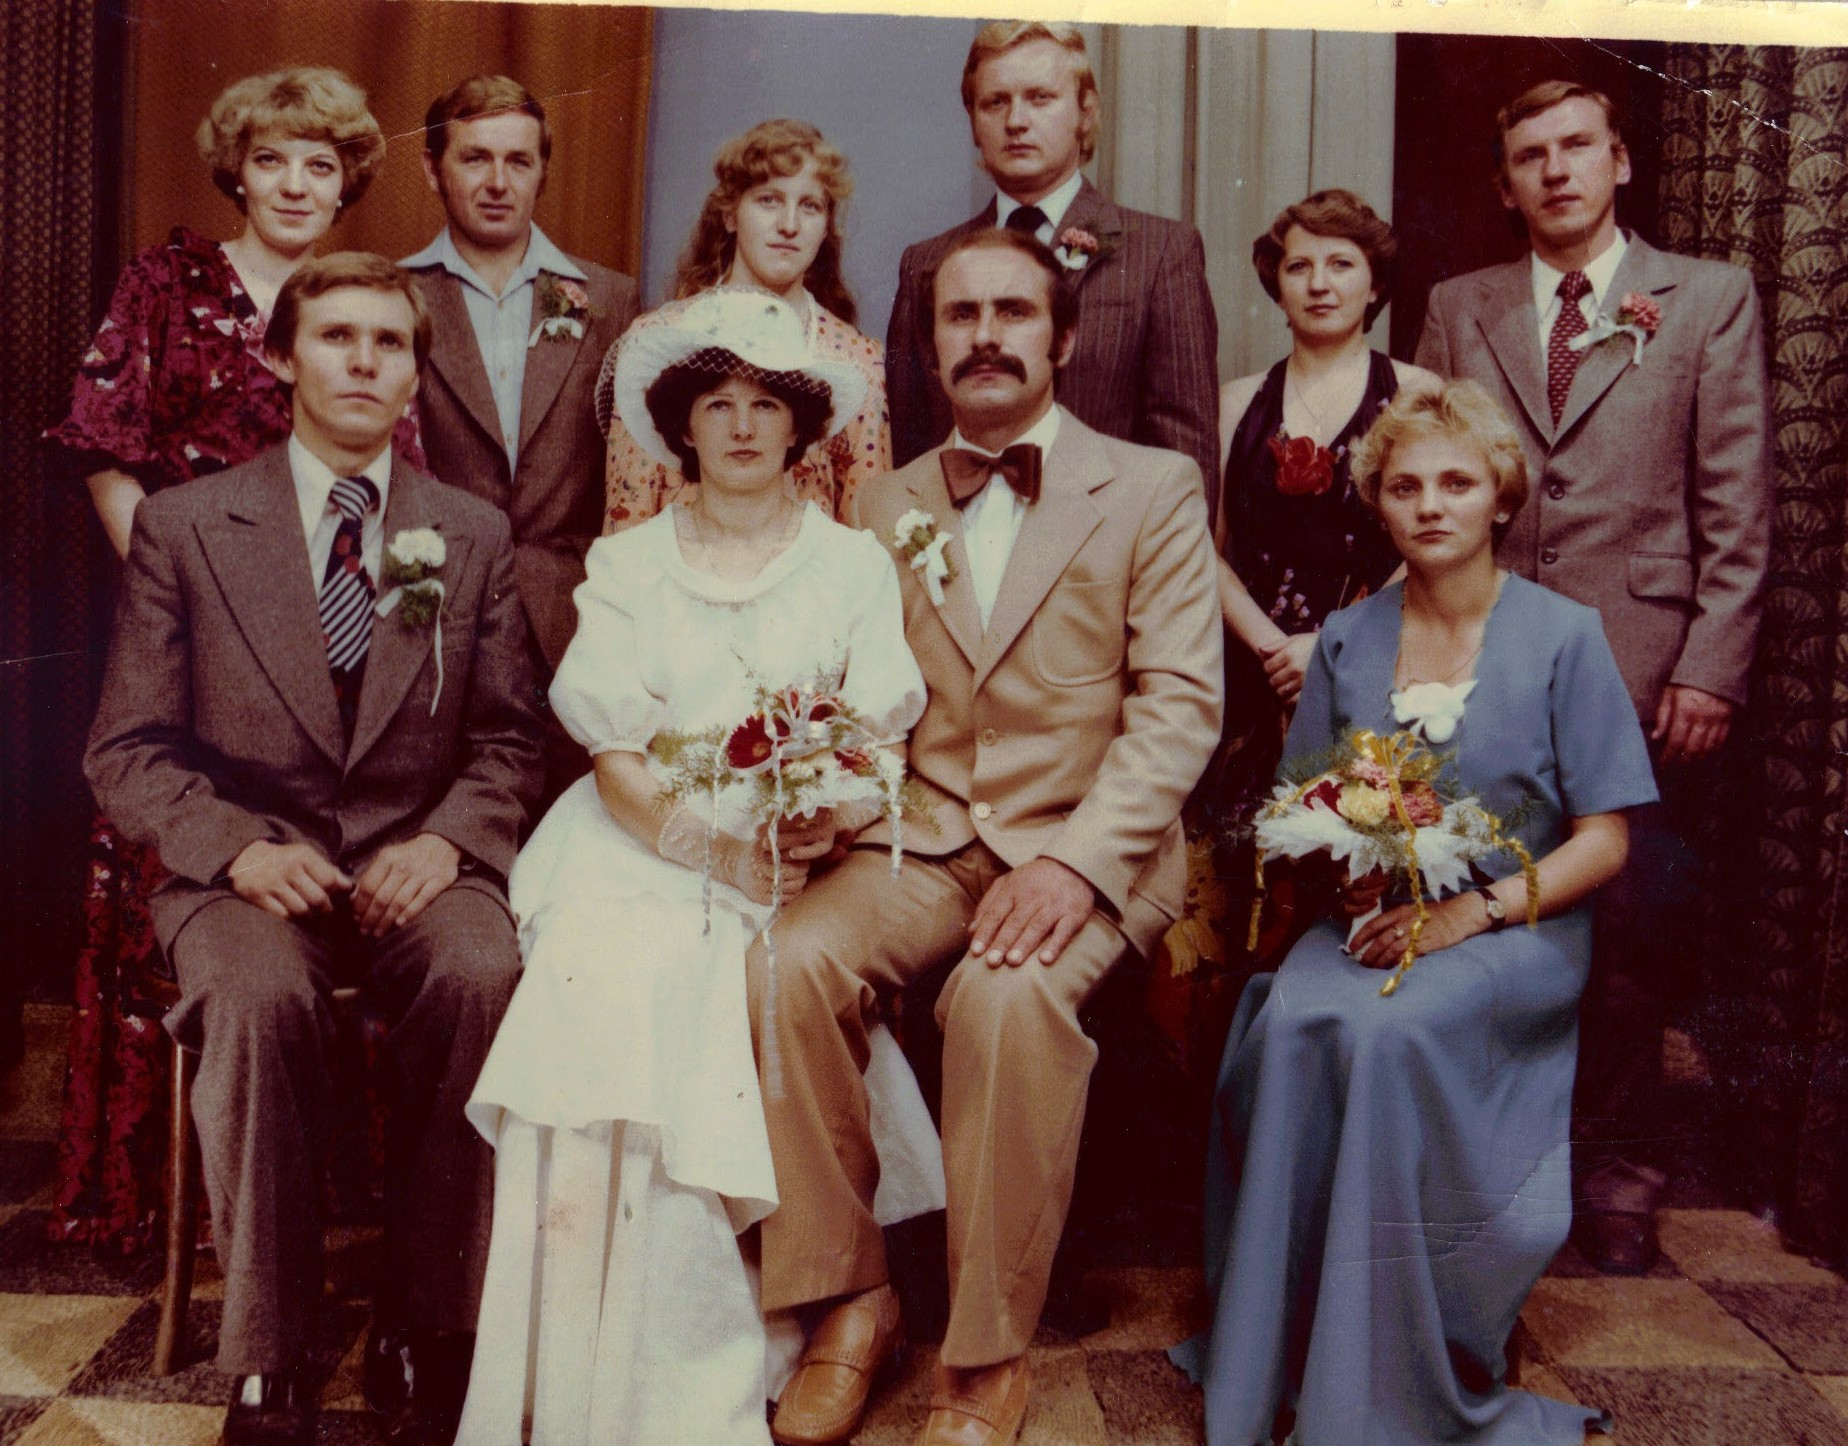
\includegraphics[width=0.7\textwidth]{zdjecia/slub_marii_gradzik_i_marka_popczyka.jpg}
\caption[Ślub Marii Gradzik i Marka Popczyka]{Ślub Marii Gradzik (prawnuczki Marianny Gradzik z domu Głąb) i Marka Popczyka. Po lewej siedzi Krzysztof Karoń, wnuczek Stanisławy Karoń z domu Głąb.}
\label{rys:slub_marii_gradzik_i_marka_popczyka}
\end{center}
\end{figure}

Najstarszy ich syn Sylwester ożenił się z Heleną Dziadkowiec (ur. 26 VII 1954 r. w Myślenicach z ojca Stanisława i matki Genowefy z domu Pajka) i ma z nią syna Marcina (ur. 21 XI 1988 r. w Krakowie).

\begin{figure}[!h]
\begin{center}
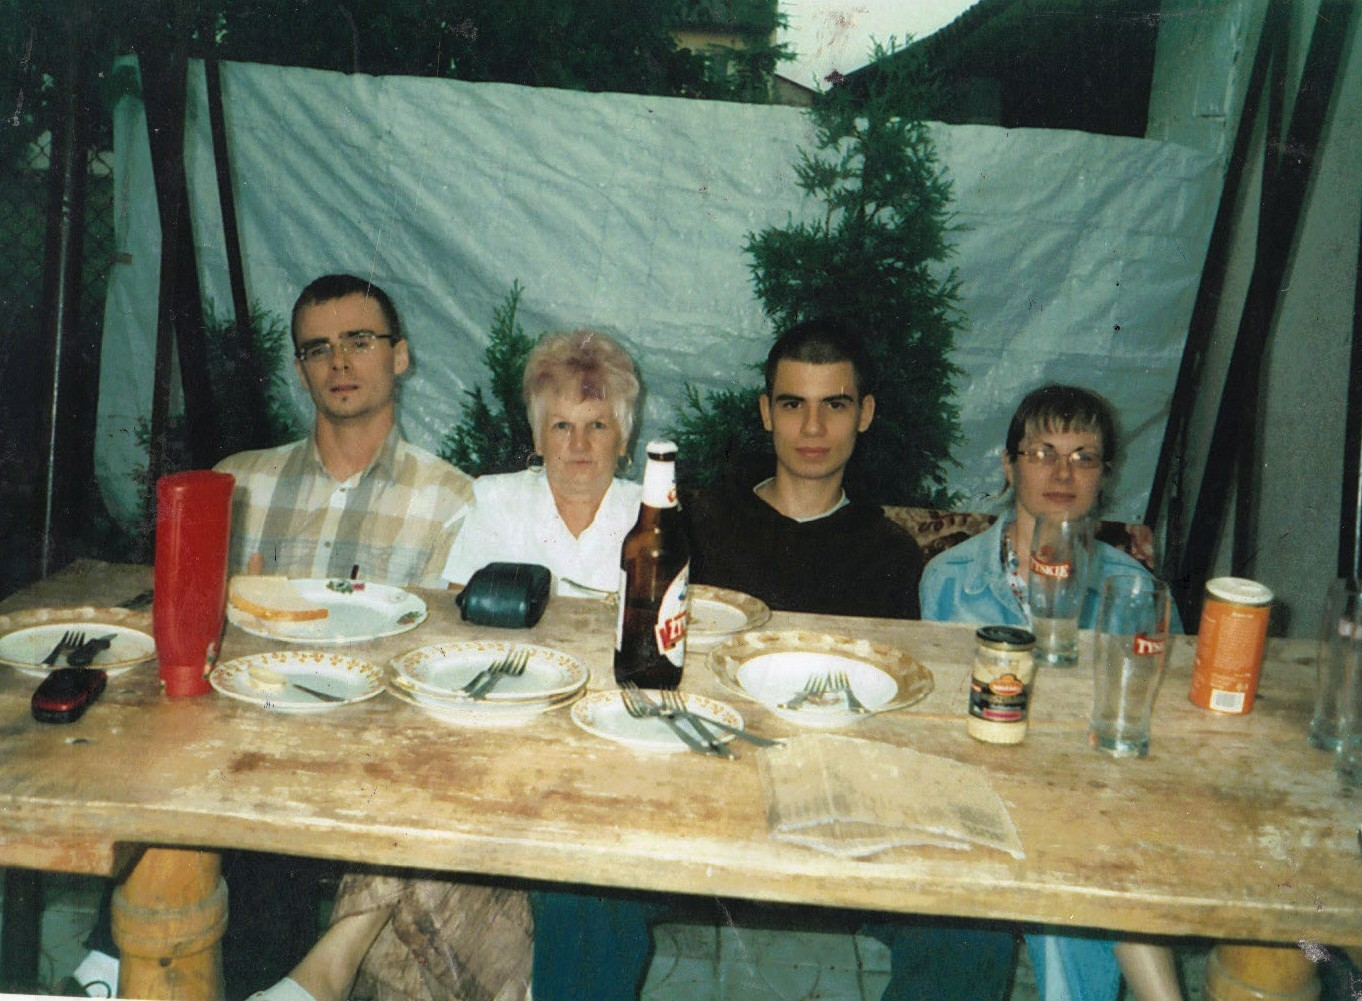
\includegraphics[width=0.6\textwidth]{zdjecia/damian_maria_ewelina_popczykowie_marcin_gradzik.jpg}
\caption[Maria Popczyk z dziećmi]{Maria Popczyk z domu Gradzik z dziećmi. Od lewej: Damian Popczyk, Maria Gradzik Popczyk, Marcin Gradzik (syn Sylwestra) oraz Ewelina Popczyk}
\label{rys:damian_maria_ewelina_popczykowie_marcin_gradzik}
\end{center}
\end{figure}

Ich drugi syn Leszek ożenił się z Barbarą Jakubczyk (ur. 18 XI 1955 r. w~Myszkowie z ojca Józefa i matki Leokadii z Czerneckich), z którą ma dwie córki: Żanetę (ur. 2 X 1984 r.) oraz Karinę (ur. 24 III 1989~r.) (rys.~\ref{rys:leszek_barbara_karina_zaneta_gradzik}).

\begin{figure}[!h]
\begin{center}
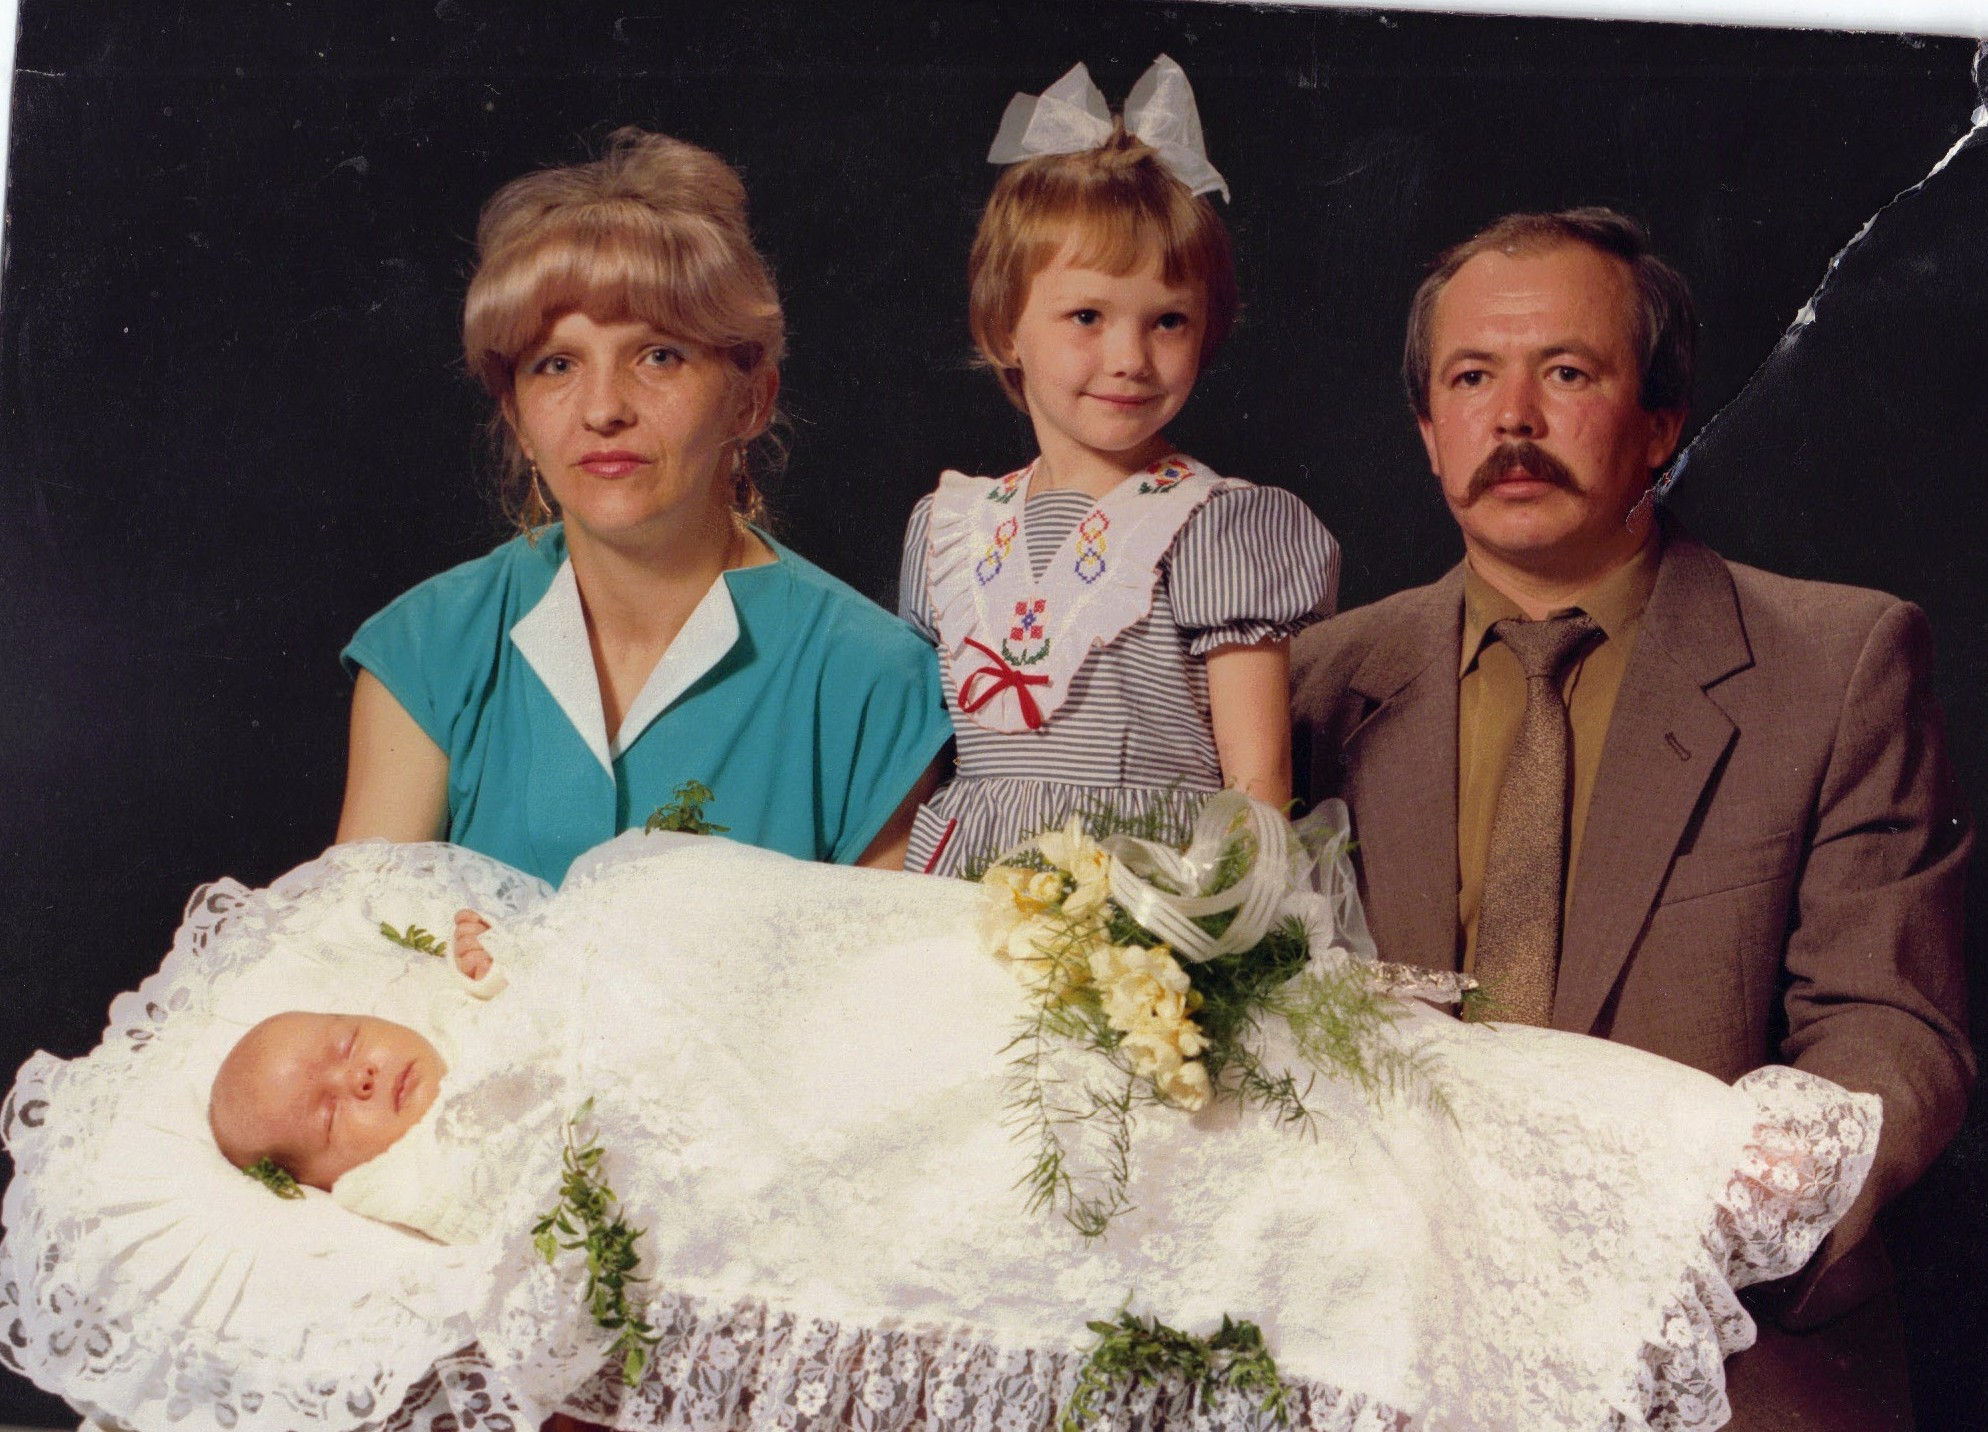
\includegraphics[width=0.6\textwidth]{zdjecia/leszek_barbara_karina_zaneta_gradzik.jpg}
\caption[Chrzest św. Kariny Gradzik]{Chrzest św. Kariny Gradzik. Na zdjęciu z rodzicami Barbarą i Leszkiem Gradzikiem (wnukiem Marianny Gradzik z domu Głąb) oraz starszą siostrą Żanetą.}
\label{rys:leszek_barbara_karina_zaneta_gradzik}
\end{center}
\end{figure}

\begin{figure}[!h]
\begin{center}
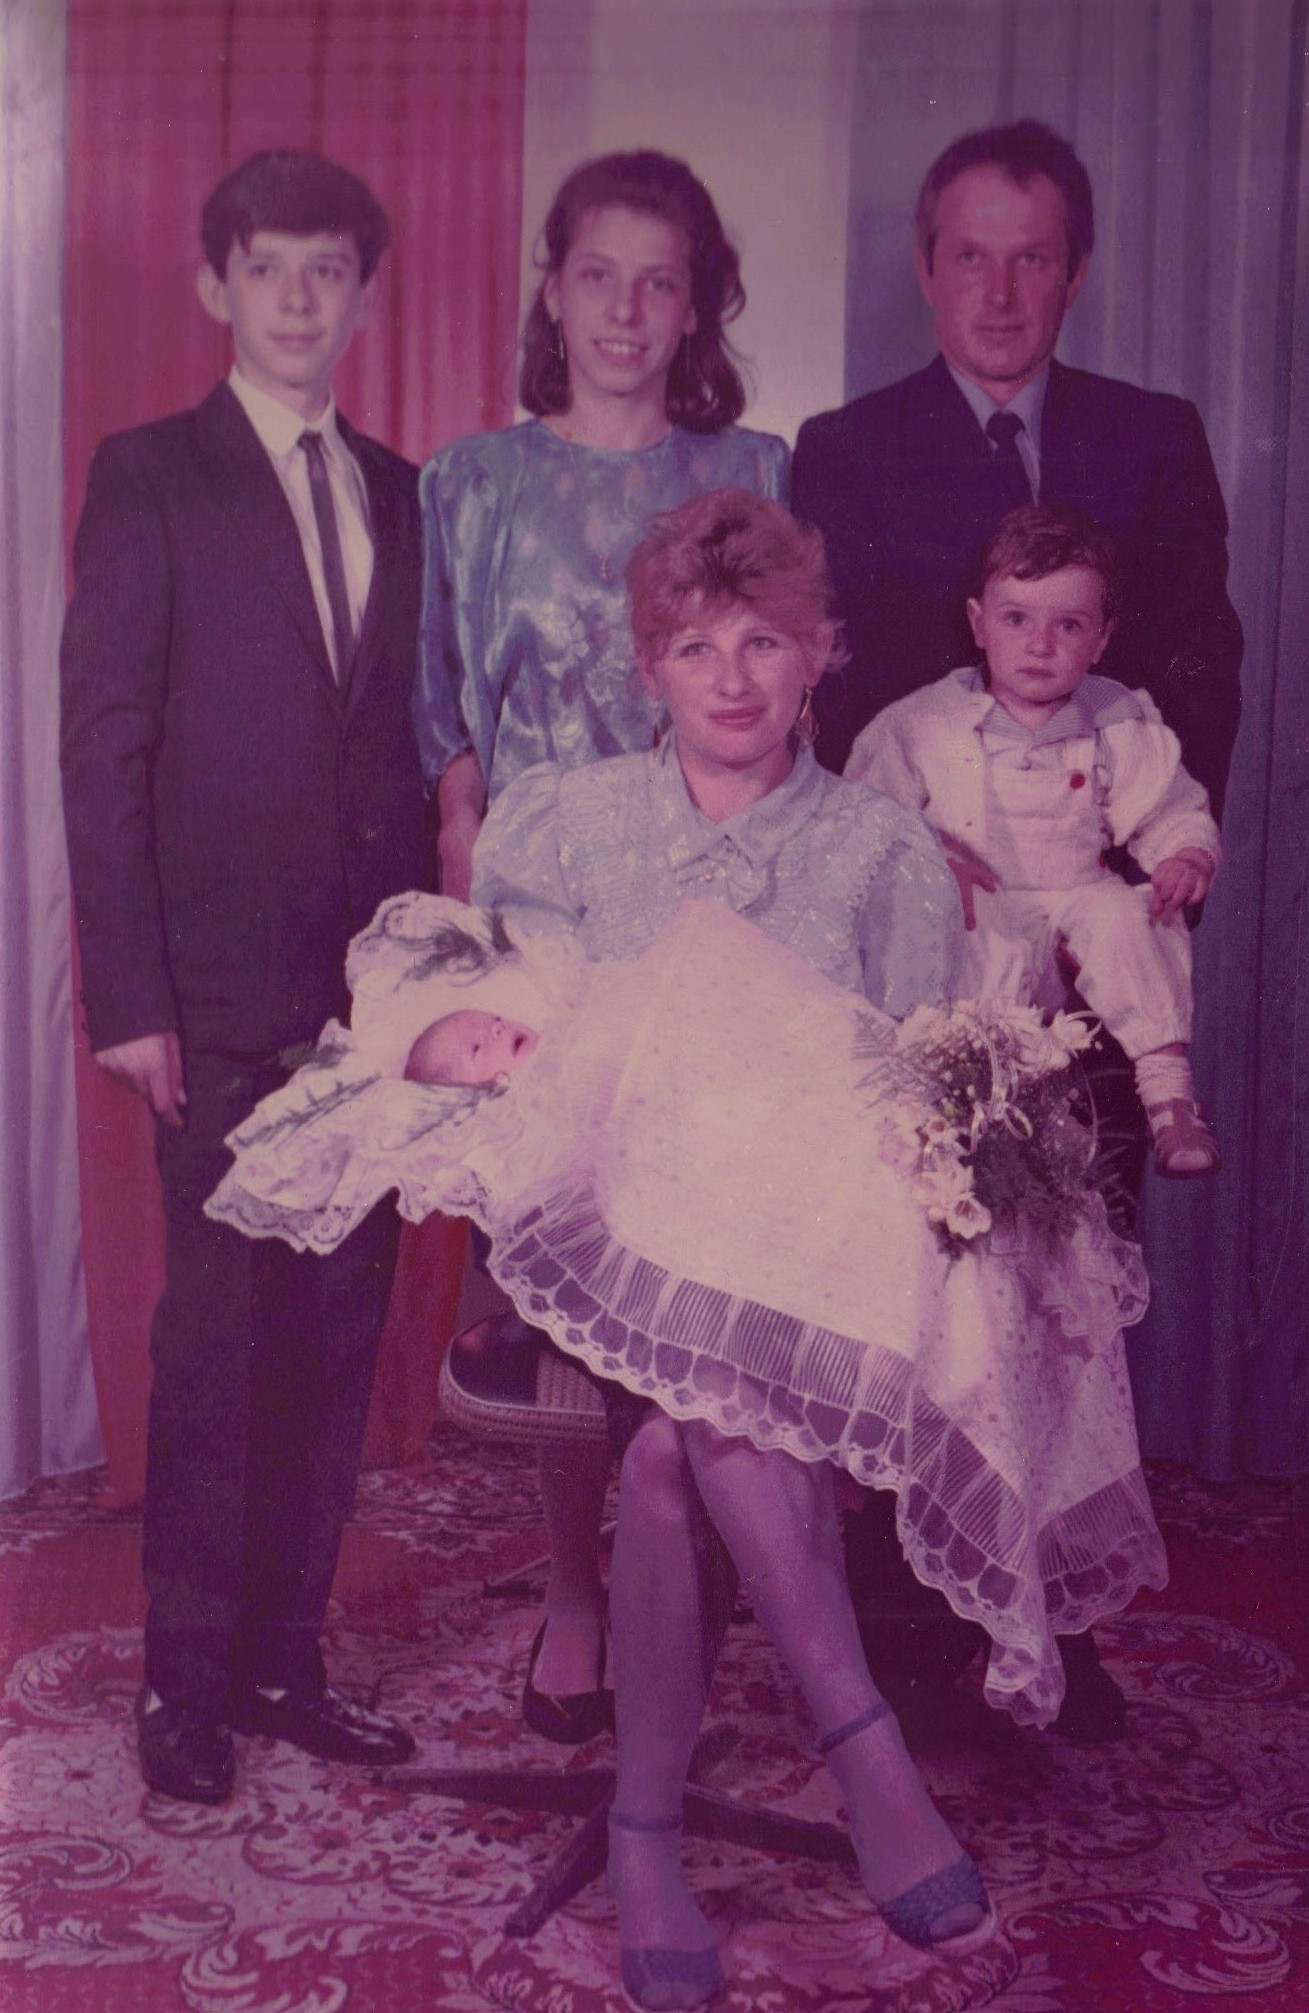
\includegraphics[width=0.43\textwidth]{zdjecia/chrzest_angeliki_gradzik.jpg}
\caption[Chrzest św. Angeliki Gradzik]{Na zdjęciu od prawej Krzysztof Gradzik (wnuk Marianny Gradzik z domu Głąb) na ręku z synem Krystianem, rodzice chrzestni oraz Anna Gradzik trzymająca do Chrztu~św. Angelikę.}
\label{rys:chrzest_angeliki_gradzik}
\end{center}
\end{figure}

Ich trzeci, najmłodszy syn Krzysztof Gradzik ożenił się z Anną Mazanek (ur. 5 VII 1963 r. w Ślęzanach z ojca Józefa i matki Stefanii z domu Błoch), z którą ma syna Krystiana (ur. 7 X 1988 r.) oraz córkę Angelikę (ur. 24 IV 1990 r.) (rys.~\ref{rys:chrzest_angeliki_gradzik}).




\section{Władysław Zygmunt Maciąg}
Marianna Głąb Gradzik po śmierci swego męża Sylwestra (zmarł dnia 16 III  1932 r. w Mirowie) wyszła powtórnie za Jana Maciąga, także wdowca po Eleonorze z Ladów (ur. 2 VIII 1907 r. w Krasawie, syna Jana i Zofii z Dzierżyków), z którym miała syna Władysława Zygmunta (ur. 2 VIII 1936 r. w Mirowie).


Ów Zygmunt (na ryc.~\ref{rys:pawel_skowronek_1_komunia}, pierwszy z prawej) ożenił się 9 V 1954 r. w Niegowie z Jadwigą Rozalią Kołacz (ur.12 IX 1932 r. w Niegowie, córką Wojciecha i Marianny z Kaimów), z którą ma dwie córki: Jolantę Jadwigę ur. 2 II 1955 r. w Niegowie oraz Bożenę Marię ur. 15 III 1958 r. także w Niegowie. Bożena Maciąg wyszła za Krzysztofa Kosa, a Jolanta wyszła dnia 9 X 1976 r. w Częstochowie za Waldemara Daniela i pewnie mieszkają w Częstochowie. Żona Zygmunta Maciąga nie żyje. Władysław Zygmunt po śmierci żony Jadwigi powtórnie się ożenił dnia 25 I 1995r. w Siedlcu Dużym z Marią z Janickich Wachowiczową.

Marianna Głąb Gradzik Maciąg zmarła 22 X 1949 r. w Mirowie. Jan Maciąg, jej drugi mąż zmarł dnia 8 VIII 1987 r. w Mirowie

Niedługo po śmierci swej najstarszej córki -- Marianny, bowiem już 17 XI 1949 r. w Mirowie zmarł nestor rodu - Walenty Głąb. Pogrzeb jego odbył się 19 XI na cmentarz w Niegowie. W 10 lat po nim zmarła Antonina z Łyszczarzów Głąbowa, jego żona i matka wszystkich tych, których tu wymieniam. Nestorka opisywanego tu rodu Głąbów zmarła 7 IX 1959 r. w Mirowie, a pogrzeb odbył się 9 września na cmentarz niegowski.
